\documentclass[a4paper,openright,12pt]{book}
\usepackage[spanish]{babel}
\usepackage{anysize}
\usepackage{cite}
\usepackage{graphicx} 
\usepackage[utf8]{inputenc}
\usepackage{multicol}
\usepackage[hidelinks]{hyperref} 
\usepackage{multirow}
\usepackage{amsmath}
\usepackage{float}
\setcounter{secnumdepth}{3} % para que ponga 1.1.1.1..
\setcounter{tocdepth}{4} % para que añadir las secciones en el índice...
\pagenumbering{Roman}


\begin{document}

\begin{titlepage}

\begin{center}
\vspace*{-1in}         
\begin{center}


\includegraphics[width=110px, height=120px]{ulalogo.png}\\
\end{center}


\vspace*{0.15in}
FACULTAD DE CIENCIAS\\
\vspace*{0.15in}
DEPARTAMENTO DE FÍSICA \\
\vspace*{0.6in}
\vspace*{0.2in}
\begin{Large}
\textbf{Desarrollo de una aplicación web para modelar la función dieléctrica a partir del análisis variacional Kramers Kronig restringido}\\

\end{Large}
\vspace*{0.3in}
\vspace*{0.3in}
\rule{80mm}{0.1mm}\\
\vspace*{0.1in}

\begin{large}
Autor: Br.Golfredo Perez Fernandez\\
Tutor: Dr.Adan Lopez\\
Cotutor: Ing.Fracisco Hidrobo 
\end{large}

\end{center}

\end{titlepage}
\tableofcontents % indice de contenidos


\pagenumbering{arabic}

\newpage

\chapter{}
\section{Introducción}

Desde los tiempos de Euclides, la interaccion de la luz con materia ha interesado a poetas, pintores y fisicos. Este interes no va mas alla de nuestra curiosidad por los materiales en si mismos, y tambien en sus aplicaciones, que podrian ser para la exploracion de estrellas distantes o el descubrimiento de nuevos pigmentos .

La interaccion entre una onda electromagnetica y un medio material puede describirse, desde un punto de vista macroscopico, mediante los llamados parametros opticos, relacionados con la funcion dielectrica del material. 

El objetivo principal del proyecto es desarrollar una aplicación Web que permita el modelar la funcion dielectrica via análisis variacional Kramers Kronig restringido a cantidades ópticas medibles. En particular se vera como obtener la función dieléctrica a partir de medidas de reflectancia que son usualmente obtenidas por la configuración experimental de radiación a incidencia normal a una superficie de material. Por lo que es necesario estudiar el fenómeno que ocurre cuando la luz interactúa con la materia, el cual esta descrito por las ecuaciones de Maxwell. Se mostrara como a partir de la función dieléctrica se deducen algunas cantidades del espectro óptico como la conductividad óptica $\sigma(w)$ , el índice de refracción $n(w)$, el coeficiente de extinción $k(w)$, la tramitancia $T(w)$ y Absorbancia  $A(w)$.

En la actualidad existen muy pocas herramientas que permitan el modelado de datos opticos por medio de esta tecnica y son software de escritorio. Esto sera de gran utilidad a diversos cientificos físicos, químicos, astronomos y cualquiera que utilice técnicas ópticas para estudiar materiales, ya que en la función dieléctrica esta contenida la información de los materiales y permite estudiar la estructura de bandas electrónicas, bandas fononicas, frecuencias fundamentales, vibraciones de red, excitones etc. 

Para lograr esto la aplicacion web estara construida con tecnologia web de nueva generacion como lo es ReactJS, Relay y GraphQL construidas y mantenidas y creadas por facebook y que ademas son la base de muchas aplicaciones web de esta epoca como lo es el mismo facebook, instagram, netflix, entre otras.

Este trabajo se dividirá en los siguientes capítulos. El capitulo 1, comprende el planteamiento del problema,  objetivos,justificación e importancia del proyecto, limitaciones, y la metodología de desarrollo. El segundo capitulo los antecedentes y bases teóricas  necesarias para la comprensión del fenómeno.  
\section{Planteamiento del Problema}


La interaccion de la radiacion y la materia es compleja pero la de la respuesta de los solidos en la posicion $r$ y en el tiempo $t$ a un campo electrico $E(r^{'},t^{'})$ en la posicion $r^{'}$ y tiempo $E(r^{'},t^{'})$  puede ser escrita como:

\begin{equation}\label{plan1}
D_{i}(r,t)=\int\int \bar{\bar\varepsilon}_{ij}(r,r^{'},t,t^{'}) E_{j}(r^{'},t^{'})dt^{'}dr^{'}
\end{equation}
Donde $i$ y $j$ se refiere a las componentes del campo electrico, desplazamiento electrico $D$ y el tensor dielectrico $\bar{\bar\varepsilon}$. 

En solidos Homogeneos la respuesta solo depende de la distancia $r-r^{'}$ mientras el tiempo es una variable continua, por lo que la ecuacion \ref{plan1} se reduce:
\begin{equation}
D_{i}(r,t)=\int\int \bar{\bar\varepsilon}_{ij}(r-r^{'},t-t^{'})E_{j}(r^{'},t^{'})dt^{'}dr^{'}
\end{equation}
La respuesta es lineal por lo que el vector desplazamiento $D$ es proporcional al campo electrico aplicaco $E$(la respuesta ocurre a la misma frecuencia del campo). En el caso de un campo electrico $E$ oscilante :  
\begin{equation}
E(r,t)=E_{0}exp{i(q\cdot r-wt)}
\end{equation}
Podemos escribir el desplzamiento electrico D en terminos de la frecuencia usando transformadas de Fourier, entonces da:
 

\begin{equation}
D_{i}(q,w)=\bar{\bar\varepsilon}_{ij}(q,w)E_{j}(q,w)
\end{equation}
Con el tensor dielectrico complejo dador por un vector de onda $q$ y frecuencia $w$. 

Por ahora solo se menejaran redes cubicas por lo que el tensor dielectrico sera una cantidad compleja $\hat{\varepsilon}$ que llamaremos funcion dielectrica. Ademas tambien la respuesta de los solidos puede estar descrita en terminos de una corriente en la posicion $r$ y en el tiempo $t$ y asi:
\begin{equation}
J(r,t)=\int\int\hat{\sigma}(r,r^{'},t,t^{'})E(r^{'},t^{'})dt^{'}dr^{'}
\end{equation}
Con el tensor conductividad complejo $\sigma(q,w)$ en respuesta a campos electricos sinusoidales  variantes en el tiempo.

De las ecuaciones de Maxwell estas dos funciones de respuesta estan relacionadas entre si por:
\begin{equation}
\hat{\varepsilon}(q,w)=1+\dfrac{4\pi i}{w}\hat{\sigma }(q,w)
\end{equation}
Excepto para algunos casos la variacion espacial de estas cantidades es identica:
\begin{equation}
\dfrac{J(r)}{E(r)}=\hat{\sigma }
\end{equation}
y con:
\begin{equation}
\dfrac{D(r)}{E(r)}=\hat{\varepsilon}
\end{equation}
Dos cantidades espacialmente independientes. Esto quiere decir que las transformadas de Fourier de $\hat{\varepsilon}$ y $\hat{\sigma}$ no tienen componentes $q\neq 0$. Existen  excepciones a cantidades en otras escalas de longitud pero usando estas restricciones se puede escribir cantidades escalares independientes de $q$:
\begin{equation}\label{varepsi}
\hat{\sigma}(w)=\sigma_{1}(w)+i\sigma_{2}(w)
\end{equation}
\begin{equation}
\hat{\varepsilon}(w)=\varepsilon_{1}(w)+i\varepsilon_{2}(w)
\end{equation}
Entonces en la funcion dielectrica y conductividad electrica esta contenida la informacion sobre la respuesta de los materiales a campos electricos, por lo que no tomaremos en cuenta efectos magneticos ya que no trateremos materiales magneticos. La dependencia en la frecuencia es llamada dispersion y de consideraciones que involucran causalidad la parte real e imaginaria de las funciones de respuesta en optica estan vinculadas mediante las relaciones Kramers Kronig y en el caso de la funcion dielectrica son:

\begin{equation}\label{varepsi1}
\varepsilon_{1}(w)-1=\frac{2}{\pi}\wp \int_{0}^{\infty}\frac{x\varepsilon_{2}(w)}{x^{2}-w^{2}}dx
\end{equation}
\begin{equation}\label{varepsi2}
\varepsilon_{2}(w)=\frac{-2w}{\pi}\wp\int_{0}^{\infty}\frac{\varepsilon_{1}(w)}{x^{2}-w^{2}}dx+\frac{4\pi\sigma_{dc}}{w}
\end{equation}

Donde $\sigma_{dc}$ es la conductividad dc, y el símbolo $\wp$ significa el valor principal de la integral de Cauchy. 

Existen maneras experimentales de extraer $\varepsilon_{1}$  y $\varepsilon_{2}$ directamente del experimento como es el caso de elipsometria. Pero existen otros experimentos que están basados en las relaciones Kramers Kronig para extraer información del espectro, como es el caso del análisis Kramers Kronig al espectro de reflectividad por radiación a incidencia normal. 

La idea de este metodo es el siguiente. Primero las ecuaciones \ref{varepsi1} y \ref{varepsi2} no pueden ser aplicadas directamente ya que $\varepsilon_{1}$  y $\varepsilon_{2}$  dependen de una fase desconocida $\phi$ dada por reflectividad compleja \cite{constrained}
\begin{center}

\begin{equation}\label{reflectividad}
r(w)=\frac{1-\sqrt{\varepsilon(w)}}{1+\sqrt{\varepsilon(w)}}=\sqrt{R(w)}exp\{i\phi(w)\}
\end{equation}

\end{center}
Se puede escribir una relación similar a \ref{varepsi} con respecto a la función de reflectividad compleja \cite{constrained}:
\begin{equation}
ln\hat{r}(w)=ln\sqrt{R(w)}+i\phi(w)
\end{equation}
De esta forma podemos escribir la relación \ref{varepsi2}  y usarla para calcular $\phi(w)$ a partir de R(w).

\begin{equation}\label{phi}
\phi(w)=\frac{-2w}{\pi}\wp\int_{0}^{\infty}\frac{ln\sqrt{R(x)}}{x^{2}-w^{2}}dx+\phi(0)
\end{equation}

Habiendo encontrado la fase $\phi$ es posible invertir la ecuación \ref{reflectividad}, y así determinar la conductividad compleja y la función dieléctrica: \cite{OpticalTechniques}

\begin{equation}
\sigma_{1}(w)=\frac{w}{4\pi}\varepsilon_{2}(w)=\frac{w}{4\pi}\frac{4\sqrt{R(w)}[1-R(w)]sin\phi_{r}}{[1+R(w)-2\sqrt{R(w)cos\phi_{r}}]^{2}}
\end{equation}
\begin{equation}
\sigma_{2}(w)=\frac{w}{4\pi}[1-\varepsilon_{1}(w)]=\frac{w}{4\pi}(1-\frac{[1-R(w)]^{2}-4R(w)sin^{2}\phi_{r}}{[1+R(w)-2\sqrt{R(w)}cos\phi_{r}]^{2}})
\end{equation}

Desafortunadamente este tratamiento basado en ecuaciones como \ref{phi} no es universal. Se ha demostrado que estas relaciones se mantienen para el caso de incidencia normal a la superficie pero dejan de cumplirse por ejemplo para la reflectividad fuera del ángulo normal a la superficie, y el mismo problema ocurre para otros casos. Por lo que es mejor tener desde el punto de vista practico una formulación mas general que pueda ser usado para diferentes configuraciones experimentales sin mayor adaptación \cite{constrained}.

El análisis Kramers Kronig restringido es una técnica que consiste en el modelado de datos experimentales, que utiliza una función matemática modelo que representa cualquier valor experimental. En nuestro caso representaremos la reflectancia R(w) medida en un limitado rango de frecuencias. 

No se puede negar que las aplicaciones de escritorio han importantes en el mundo de la computacion ya que se han utilizado desde hace mucho tiempo aunque a medida que nos actualizamos se han ido utilizando las aplicaciones web las cuales se han vuelto muy importantes debido a las ventajas que ofrecen, especialmente porque van dirigidas a gran cantidad de personas sin necesidad de descargar la misma en el ordenador.
Por ello se ha decidido construir una aplicacion web que implemente el analisis variacional Kramers Kronig restringido.


\section{Objetivo General}

\begin{itemize}
\item Desarrollar una aplicación Web que implemente el análisis variacional Kramers-Kronig restringido para modelar la función dieléctrica compleja de los solidos.
\end{itemize}

\section{Objetivos Específicos}
\begin{itemize}
\item Realizar la descripción formal del análisis variacional Kramers-Kronig restringido.
\item Determinar los requerimientos de la aplicación Web para la implementación del análisis.
\item Construir la aplicación Web que implemente el análisis variacional Kramers-Kronig restringido.
\item Comprobar los resultados del análisis.
\item Realizar la implantación del sistema.
\end{itemize}


\section{Justificación e Importancia del Proyecto}

Los resultados obtenidos experimentalmente en espectroscopia son muy útiles en la caracterización de materiales permitiendo determinar la naturaleza del material y posibles aplicaciones. Dependiendo rango de frecuencia con que se esta estudiando una muestra de material se puede obtener información sobre la estructura de bandas electrónica o fononicas del material. Por ejemplo si se hacen mediciones de reflectancia a incidencia normal en el rango de frecuencia infrarrojo la obtención de la función dieléctrica permite estudiar la estructura fononica y así los niveles energéticos de los materiales\cite{SolidStatePhysics}. 

Es importante toda la serie de propiedades ópticas que se desprenden de la función dieléctrica como el índice de refracción que esta determinado por el cambio de la velocidad de la onda en el medio y coeficiente de extinción que describe la absorción de la onda en el medio, ambos coeficientes determinan la propagación de la onda electromagnética en el medio.  

El modelado de la función dieléctrica a partir del análisis variacional Kramer-Kronig restringido es un enfoque que ignora el uso de modelos(Drude Lorentz, Fano, Tauc-Lorentz etc.) para ajustarse al tipo de datos, en vez de eso es una técnica que se adapta prácticamente a cualquier tipo de medición óptica. 

Por medio de una aplicacion Web los investigadores podrán acceder rápidamente a una herramienta capaz de modelar  la funcion dielectrica a partir de cualquier cantidad  del espectro optico de los solidos que describa fenómenos físicos causales en óptica y que cumplan con las relaciones Kramers Kronig de forma rápida y en tiempo real. La construcción de una aplicación web tendrá múltiples ventajas como el ahorro de tiempo, la compatibilidad y la portabilidad que ofrece ya que se puede acceder desde cualquier dispositivo y evita el uso de recursos de sistema por parte del usuario, que por el contrario en el caso de los programa de escritorio la velocidad de respuesta del programa dependerá de las características propias de cada computador.\\


\section{Alcances y Limitaciones}

Existen restricciones importantes en esta técnica de análisis. Lo primero es que los datos experimentales deben cubrir un amplio rango de frecuencias. Segundo, esta técnica puede ser solo aplicada a funciones que cumplan con las relaciones Kramers-Kronig \cite{electrodynamics}. 

\section{Metodología}
Actualmente existen un gran variedad de metodologías para desarrollar programas basadas en enfoques generales que han ido evolucionando. En nuestro caso utilizaremos la metodología en Cascada considerada como una de las mas antiguas y su nombre se debe al lineamiento de procesos para hacer funcionar el sistema. Veamos cuales son sus fases de desarrollo:\cite{ingsof}
\begin{itemize}
\item Análisis y definición de requerimientos: Los servicios, restricciones y metas del sistema son definidas a partir de consultas con los científicos.

\item Diseño del Programa: Se establece la arquitectura del sistema. Aquí se identifican las abstracciones fundamentales de la aplicación Web y sus relaciones.
\item Diseño Algorítmico y Codificación: En esta fase es momento de escribir el código necesario de la aplicación Web.
\item Integración y Verificación del Sistema: Los programas o unidades son integradas como un sistema completo para asegurar que se cumplan con los requerimientos del programa. Después de las pruebas, el sistema es entregado al cliente.
\item Funcionamiento y Mantenimiento: Por lo general esta fase es la mas larga del ciclo de vida. El sistema se instala y se pone en funcionamiento practico. El mantenimiento implica corregir errores no descubiertos en las etapas anteriores del ciclo de vida, mejorar la implementación de las unidades del sistema y resaltar los servicios del sistema una vez que se descubren nuevos requerimientos.
\end{itemize} 


\chapter{Marco Teórico}

\section{Antecedentes}

En las ultimas décadas se han desarrollado programas de escritorio como OPTPAL o mas recientemente RefFit(Construido por Alexey Kuzmenko) que permiten analizar el espectro ópticos de los sólidos.  RefFit es un software potente compacto e interactivo para Windows 95,98,NT,XP diseñado para modelar el espectro óptico a partir de mediciones de reflectividad, transmisión, elipsometría etc. Utiliza modelos de funciones dieléctricas como el Drude-Lorentz, Fano, Tauc-Lorentz y muchos otros, formando  una rica biblioteca de modelos, tiene un motor basado en el algoritmo de Levenberg-Marquard y permite ajustar manual o automáticamente varios conjuntos de datos de diferentes tipos.\cite{guide}.
\section{Clasificación de los procesos ópticos}

La luz interactúa con los materiales de muchas maneras, los metales son brillantes, el agua es transparente, los vitrales y piedras preciosas  transmiten hermosos colores. Por lo que a continuación se estudiara el fenómeno óptico que ocurre cuando la luz interactúa con los materiales del estado solido. 

En esta y en las próximas secciones se estará clasificando el fenómeno y determinando los coeficientes que se utilizan para cuantificarlo. También se introducirán algunos materiales y las diferencias de como difieren el estado solido de la fase liquida y gaseosa.

El amplio rango de propiedades ópticas observadas en el estado solido pueden ser clasificadas en la reflexión, propagación y transmisión de la luz, en la figura \ref{procesosFigura} se ilustra un rayo de luz que viaja de un medio material ($N'$) y luego incide 
con otro medio material finito ($N$). 

\begin{center}
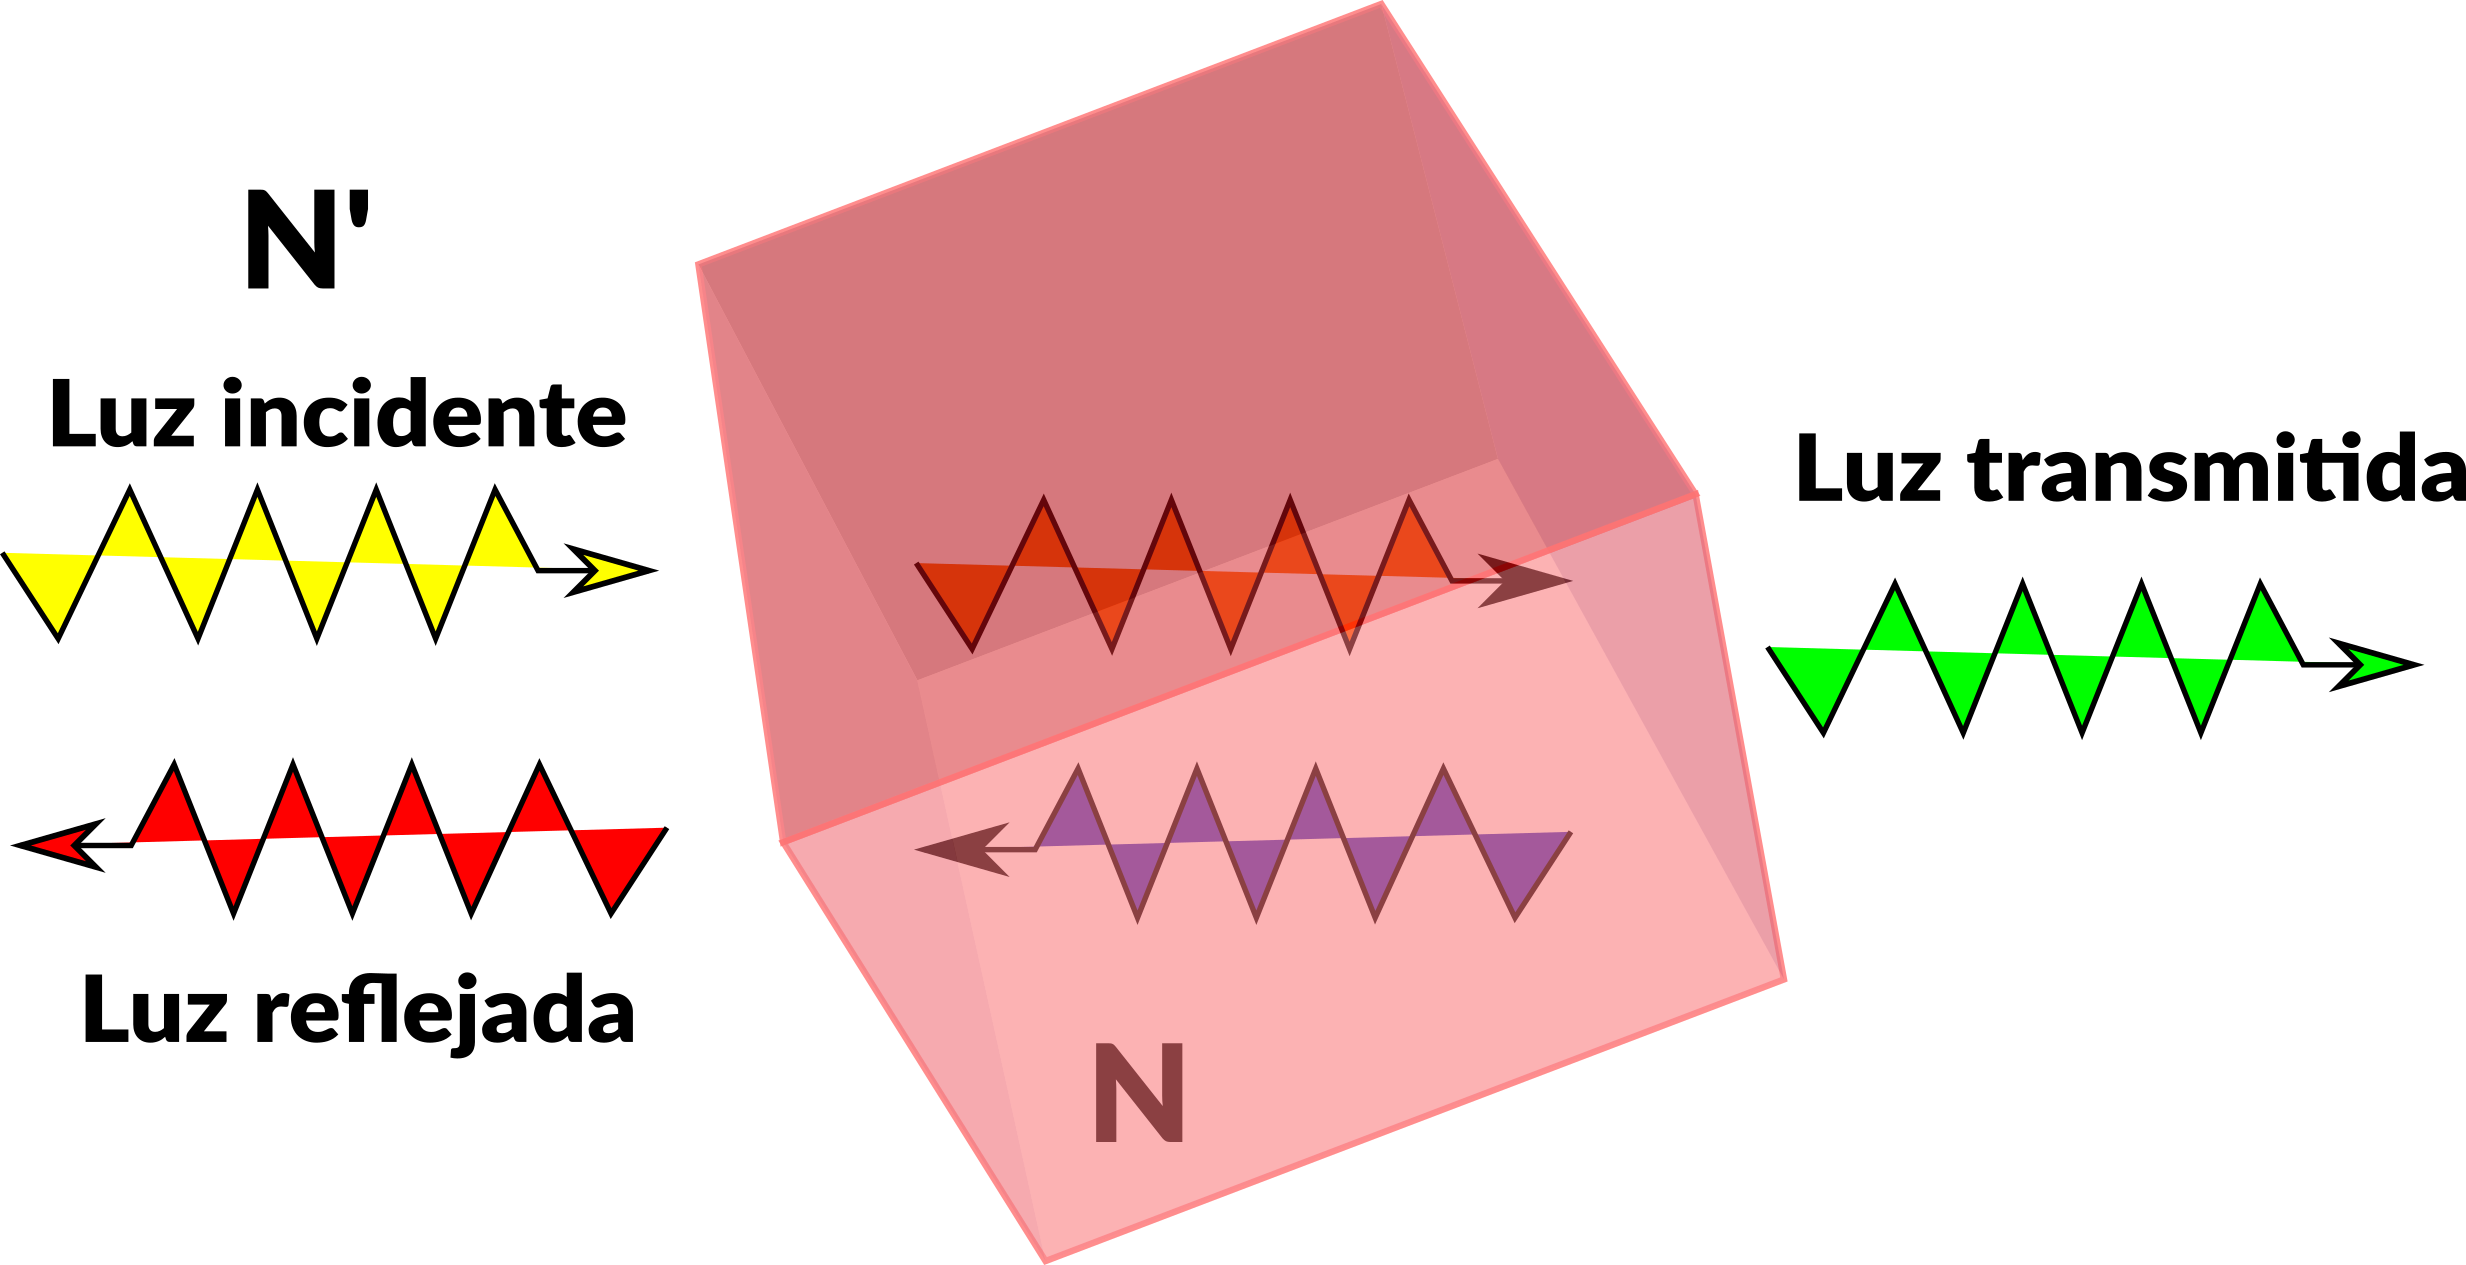
\includegraphics[width=300px, height=150px]{procesosopticos.png}\label{procesosFigura}\\

Figura \ref{procesosFigura}. Procesos ópticos.
\end{center}

Una parte de la luz es reflejada en la superficie, mientras que el resto se propaga a través del medio y luego cuando el alcanza el final del medio la luz es reflejada y transmitida nuevamente debido al cambio de interfaces. Entonces la cantidad de luz que al final es transmitida esta relacionada con las ondas reflejadas y también en la manera en que la luz es dispersada y absorbida a medida que atraviesa el medio material. Describiendo un poco mejor estos fenómenos \cite{MarkFox}:\\


\begin{itemize}
\item La refracción es el cambio de dirección que experimenta la luz cuando atraviesa la interfaz de dos medios. El cambio en la dirección es consecuencia de un cambio en la velocidad del rayo de luz cuando interactúa con un medio de propiedades ópticas distintas. La refracción en si mismo no afecta la intensidad de la luz que se propaga \cite{MarkFox}.

\item La absorción ocurre durante la propagación si la frecuencia de la luz que se propaga es resonante con la frecuencia de transición de los átomos en el medio, como consecuencia el rayo sera atenuado en el proceso. Las transmisiones de luz en el medio esta claramente relacionado con la absorción, porque solo la luz que no es absorbida sera transmitida. Las absorciones son responsables de la coloración de muchos materiales ópticos. Como por ejemplo los rubíes, son rojos porque absorben luz en frecuencias del azul y verde pero no rojo \cite{MarkFox}.

\item La dispersión es fenómeno en el cual la luz cambia de dirección y posiblemente también de frecuencia luego de interactuar con el medio. El numero total de fotones que viajan en la dirección de propagación disminuye, debido a que la luz es redirigida en otras direcciones. La dispersión sin embargo tiene el mismo efecto de atenuación en la intensidad de la onda que en la absorción. Entonces, sera inelastica si la frecuencia de la luz dispersada cambia y elástica si la frecuencia cambia en el proceso \cite{MarkFox}.

\item La luminiscencia es el nombre que se le da al proceso de emisión espontánea de la luz por átomos excitados en el estado solido y puede ocurrir durante la absorción. La luz re-emitida sera en todas las direcciones y tendrá una frecuencia diferente a la de la luz absorbida. En realidad la luminiscencia no ocurre en el instante en que se produce la absorción, toma una cantidad de tiempo característica volver a emitir luz por emisión espontánea. Esto significa que los átomos excitados pueden disipar energía como calor antes de que ocurra la emisión de luz.\cite{MarkFox}.
\end{itemize}

Estos fenómenos que pueden ocurrir cuando la luz se propaga a través del medio y están descritos por el campo de óptica lineal, ya que si la intensidad de la luz es muy alta, estarían descritos por la óptica no lineal. Un ejemplo seria el duplicamiento de frecuencias, en el cual la frecuencia incidente se duplica cuando interactúa con el medio.

\section{Espectro Óptico}

Con espectro óptico nos referiremos a cantidades que dependen de frecuencias y que están totalmente determinadas por la función dieléctrica del material estudiado, un ejemplo de ellas es la reflectividad $R(w)$ la cual puede ser medida directamente y otra es la conductividad óptica $\sigma(w)$ la cual usualmente no es medida directamente pero es derivada por medio de algún análisis. 

Para deducir estas cantidades se debe utilizar las  ecuaciones de Maxwell y sus  soluciones para campos eléctricos y magnéticos variantes en el tiempo. Se vera que a partir de las ecuaciones de Maxwell se pueden describir las propiedades de propagación de ondas electromagnéticas cuando la luz interacciona con la materia. Pero primero estudiemos el caso de radiación electromagnética que se propaga en el vacío donde ecuaciones de Maxwell toman la siguiente forma\cite{OpticalTechniques}:

\begin{equation}\label{0.2}
\vec{\nabla}\cdot \vec{E}(r,t)= 4\pi \rho(r,t)
\end{equation}
\begin{equation}\label{0.3}
\vec{\nabla}\cdot \vec{B}(r,t)=0
\end{equation}
\begin{equation}\label{0.4}
\vec{\nabla}\times\vec{E}(r,t)+\frac{1}{c}\frac{\partial\vec{B}(r,t)}{\partial t}=0
\end{equation}
\begin{equation}\label{0.5}
\vec{\nabla}\times\vec{B}(r,t)-\frac{1}{c}\frac{\partial \vec{E}(r,t)}{\partial t}=\frac{4\pi}{c}\vec{J}(r,t)
\end{equation}

Donde $\vec{E}$ es la fuerza del campo eléctrico, $\vec{B}$ es la densidad de flujo magnético, $\rho$ es la densidad de carga, $\vec{J}$ es la densidad de corriente, y $c=2.99792458 m/s$ es la velocidad de la luz en el vacío. La ecuación \ref{0.2} es conocida como la ley de Gauss para campos eléctricos, la ecuación \ref{0.3} como la ley de Gauss para campos magnéticos, \ref{0.4} como la inducción de Faraday y \ref{0.5} como la ley de Ampére \cite{OpticalTechniques}. 

En la presencia de un medio los campos eléctricos y magnéticos pueden generar dipolos eléctricos y magnéticos, polarizar cargas e inducir corrientes. El campo eléctrico y magnético no serán uniformes dentro del material y fluctuaran de un punto a otro reflejando la periodicidad de la red atómica. Estos campos serán diferentes comparados a que estuviesen en el vacío, por lo que consecuentemente se usa el desplazamiento eléctrico $D$ en vez de la fuerza del campo eléctrico $E$, y la inducción magnética $B$  con la fuerza del campo magnético $H$ para tomar las modificaciones creadas por el medio.

La densidad de carga total $\rho=\rho_{total}$ usada en la ley de Coulomb \ref{0.2} en presencia del medio tendrá dos términos. Para longitudes de onda apreciablemente mas grandes que el espaciamiento inter-atómico se puede considerar un valor promedio para las densidades de carga ($\rho_{externo}$), para los que no, habrá una contribución debido a la polarización debido al medio ($\rho_{polarizado}$):
\begin{equation}
\rho_{total}=\rho_{externa}+\rho_{polarizacion}
\end{equation}
con:
\begin{equation}
\rho_{polarizacion}=-\nabla\cdot P
\end{equation}

Ahora asumiendo que no hay corrientes externas presentes $J_{externa}=0$. La densidad total de corriente $J=J_{total}$ de las ecuaciones de Maxwell consiste de una contribución $J_{conduccion}$ que surge del movimiento de electrones presentes en el campo eléctrico y de una contribución $J_{ligados}$ debido a la redistribución de cargas ligadas:

\begin{equation}
J_{total}=J_{conduccion}+J_{ligados}
\end{equation}

Por medio de la ley de ohm, se puede relacionar las corrientes de conducción $J_{conduccion}$ con la conductividad del material $\sigma_{1}$ y el campo eléctrico aplicado $E$ \cite{electrodynamics}:

\begin{equation}\label{1.7}
J_{conduccion}=\sigma_{1}\vec{E}
\end{equation}

También se asumirá que no debe haber cambios debido a campos magnéticos ya que no estamos considerando efectos magnéticos. 

La polarización dependiente del tiempo $\partial P/\partial t$ y dependencia espacial de la magnetización $\nabla\times M$ contribuirían a lo que es llamado desplazamiento de corriente para cargas ligadas $J_{ligados}$. Ahora incluyendo estas consideraciones explícitamente en la ecuación de Maxwell \ref{0.4}(inducción de Faraday) se convierte:
\begin{equation}
\nabla\times B(r,t)-\frac{1}{c}\frac{\partial E(r,t)}{\partial t}=\frac{4\pi}{c}J_{total}(r,t)=\frac{4\pi}{c}[J_{conduccion}(r,t)+\frac{\partial P(r,t)}{\partial t}+c\nabla \times M(r,t)]
\end{equation}
y la ecuación \ref{0.2} cambia a :
\begin{equation}
\nabla \cdot E(r,t)=4\pi \rho_{total}(r,t)=4\pi[\rho_{externo}-\nabla\cdot P(r,t)]
\end{equation}

Estas reformulaciones de las ecuaciones de Maxwell requieren la definición del desplazamiento eléctrico $D$ y la fuerza del campo magnético $H$.


\begin{equation}\label{desplazamientoelectrico1}
D_{i}(r,t)=\int\int \bar{\bar{\varepsilon}}_{ij}(r-r^{'};t-t^{'})E_{j}(r^{'},t^{'})dt^{'}dr^{'}
\end{equation}

Donde $i$ y $j$ se refieren a las componentes del campo eléctrico $E$ y desplazamiento eléctrico $D$. El termino $\bar{\bar{\varepsilon}}_{ij}$ es llamado tensor dieléctrico complejo.

Ahora si asumimos que la respuesta sera a la misma frecuencia del campo eléctrico aplicado (respuesta lineal) y un medio isotropico (propiedades idénticas en todas direcciones), debido a esto el tensor dieléctrico $\bar{\bar{\varepsilon}}$ sera una cantidad escalar que se llama constante dieléctrica $\varepsilon_{1}$. La fuerza del campo eléctrico $E$ y el desplazamiento eléctrico(o densidad de flujo eléctrico) D están conectados por la constante dieléctrica(o permitividad) $\varepsilon_{1}$:

\begin{equation}\label{1.5}
\vec{D}(r,t)=\varepsilon_{1}(r,t)\vec{E}(r,t)=(1+4\pi\chi_{e}(r,t))\vec{E}(r,t)=\vec{E}(r,t)+4\pi \vec{P}(r,t)
\end{equation}

Con $\vec{P}(r,t)=\chi_{e}(r,t)\vec{E}(r,t)$, donde $\vec{P}$ es la polarización inducida y $\chi_{e}$ es la susceptibilidad dieléctrica del medio y $\varepsilon_{1}$ es la constante dieléctrica. La constante dieléctrica puede ser tanto positiva o negativa.

Similarmente la fuerza magnética del campo $H$ esta conectado con la inducción magnética $B$
mediante la permeabilidad $\mu_{1}$
\begin{equation}\label{1.6}
\vec{B}(r,t)=\mu_{1}(r,t)\vec{H}(r,t)=(1+4\pi \chi_{m}(r,t))\vec{H}(r,t)=\vec{H}(r,t)+4\pi \vec{M}(r,t)
\end{equation}

Donde $\chi_{m}$ es la susceptibilidad magnética y $M=\chi_{m} H$ es la magnetización. Las cantidades $\varepsilon_{1},\chi_{e},\mu_{1}$ y $\chi_{m}$ que están conectadas con los campos son sin unidades. La susceptibilidad magnética $\chi_{m}$ es típicamente cuatro o cinco ordenes de magnitud mas pequeña que la susceptibilidad eléctrica $\chi_{e}$, por esta razón se tomara $\mu_{1}=1$ ya que las propiedades magnéticas pueden ser ignoradas (excepto en ferro-magnetismo).


Ahora se definirán los coeficientes ópticos que caracterizan la propagación y disipación de la onda electromagnética en un medio material como la constante dieléctrica y la conductividad óptica y también coeficientes ópticos a mayor escala como el índice de refracción y el coeficiente de extinción. Luego se discutirá el fenómeno que ocurre en la interfaz del espacio vacío y la materia(o en general entre dos medios con diferentes constantes ópticas), esto llevara a la obtención de coeficientes ópticos accesibles experimentalmente como la reflectividad y la transmisión óptica. \cite{electrodynamics}.


Utilizando estas definiciones se pueden reescribir las ecuaciones de Maxwells en presencia de materia \cite{OpticalTechniques}

\begin{equation}\label{1.4}
\vec{\nabla}\cdot \vec{D}(r,t)=4\pi\rho(r,t)
\end{equation}
\begin{equation}\label{1.2}
\vec{\nabla}\cdot \vec{B}(r,t)=0
\end{equation}
\begin{equation}\label{1.1}
\vec{\nabla}\times \vec{E}(r,t)+ \frac{1}{c}\frac{\partial \vec{B}(r,t)}{\partial t}=0
\end{equation}
\begin{equation}\label{1.3}
\vec{\nabla}\times \vec{H}(r,t)-\frac{1}{c}\frac{\partial \vec{D}(r,t)}{\partial t}=\frac{4\pi}{c}\vec{J}(r,t)
\end{equation}

La introducción de constantes ópticas a partir de estas ecuaciones ayudaran a describir la polarización del medio debido a fuentes electromagnéticas a mayores escalas que solo tamaños atómicos, así las constantes ópticas facilitan la descripción de la interacción de ondas electromagnética y la materia \cite{OpticalTechniques}.

Utilizando  la ley de Ohm \ref{1.7}, y \ref{1.5} podemos reescribir \ref{1.3} como \cite{electrodynamics}:

\begin{equation}\label{1.8}
c\nabla\times \vec{H}(r,t)=\sigma_{1}(r,t) \vec{E}(r,t)+\frac{\partial \vec{D} (r,t)}{\partial t} 
\end{equation}
Queremos que la dependencia en el tiempo sea armónica por lo que se toma $\partial D/\partial t= -iw D$ quedando \cite{electrodynamics}:
\begin{equation}\label{1.9}
c\nabla\times \vec{H}(r,t)=4\pi \sigma_{1}(r,t) \vec{E}(r,t)-iw\varepsilon_{1}(r,t) \vec{E}(r,t) =-iw\hat{\varepsilon}(r,t) \vec{E}(r,t)
\end{equation}
Derivando así la función dieléctrica compleja   como una respuesta del material a los cambios de polarización debido a la radiación electromagnética.
\begin{equation}\label{1.10}
\hat{\varepsilon}(r,t)=\varepsilon_{1}(r,t)+i\frac{\sigma_{1}(r,t)}{w}=\varepsilon_{1}(r,t)+i\varepsilon_{2}(r,t)
\end{equation}
Ahora definida la función dieléctrica compleja se relacionara con las propiedades de propagación de la onda en el medio material. Para ello primero se utiliza la identidad vectorial \cite{OpticalTechniques} :

\begin{center}
$\vec{\nabla}\times (\vec{\nabla}\times \vec{E}(r,t))=\vec{\nabla}(\vec{\nabla}\cdot \vec{E}(r,t))-\nabla^{2}\vec{E}(r,t)$\\
\end{center}
Junto con las ecuaciones \ref{1.1} y \ref{1.4} se puede separar las componentes eléctricas y magnéticas \cite{electrodynamics} :

\begin{equation}\label{1.12}
\frac{\partial}{\partial t}(\vec{\nabla} \times \vec{B} (r,t))=\nabla^{2}\vec{E}(r,t)-\vec{\nabla}(\frac{\rho(r,t)}{\varepsilon_{1}(r,t)})
\end{equation}

Si se utiliza las ecuaciones  \ref{1.5}, \ref{1.7} y \ref{1.6} en la ecuación de Maxwell \ref{1.3} se obtiene \cite{electrodynamics}:

\begin{equation}\label{1.13}
\nabla \times \vec{B}(r,t)=\varepsilon
_{1}(r,t)\mu_{1}(r,t)\frac{\partial \vec{E}(r,t)}{\partial t}+\sigma_{1}(r,t)\mu_{1}(r,t)
\vec{E}(r,t)
\end{equation}

Combinando las ecuaciones \ref{1.12} y \ref{1.13} y además suponiendo que no hay fuentes eléctricas $\rho=0$, se determinan las ecuaciones para campos eléctricos y de manera similar para el campos magnéticos propagándose en presencia de materia \cite{electrodynamics}:

\begin{equation}\label{1.14}
\nabla^{2}\vec{E}(r,t)=\varepsilon_{1}(r,t)\mu_{1}(r,t)\frac{\partial^{2}\vec{E}(r,t)}{\partial t^{2}}+{\sigma_{1}(r,t)\mu_{1}(r,t)}\frac{\partial \vec{E}(r,t)}{\partial t}
\end{equation}

\begin{equation}\label{1.15}
\nabla^{2}\vec{H}(r,t)=\varepsilon_{1}(r,t)\mu_{1}(r,t)\frac{\partial^{2}\vec{H}(r,t)}{\partial t^{2}}+\sigma_{1}(r,t)\mu_{1}(r,t) \frac{\partial \vec{H}(r,t)}{\partial t}
\end{equation}

Una solución para estas ecuaciones considerando un medio infinito para obviar efectos de borde tenemos que para campos eléctricos y magnéticos \cite{electrodynamics}:

\begin{equation}\label{1.16}
   \vec{E}(r,t)=E_{0}e^{i(\vec{q}(r,t)\cdot r-wt)}
\end{equation}

\begin{equation}\label{1.17}
   \vec{H}(r,t)=H_{0}e^{i(\vec{q}(r,t)\cdot r-wt-\phi(r,t))}
\end{equation}

El factor $\phi$ indica que los campos eléctricos y magnéticos pueden estar en fases distintas, debido a que existe un medio material ($\sigma_{1}\not= 0$). Como veremos a continuación el vector $\vec{q}$
es una cantidad compleja, que describe la dependencia espacial de la onda y toma en cuenta la propagación y la atenuación de la onda \cite{electrodynamics}. Sustituyendo la solución \ref{1.16} en la ecuación \ref{1.14}, encontramos la siguiente relación para $q$:

\begin{equation}\label{1.18}
\vec{q}(r,t)=\frac{w}{c}[\varepsilon_{1}(r,t)\mu_{1}(r,t)+ \frac{i4\pi\mu_{1}(r,t)\sigma_{1}(r,t)}{w}]^{1/2}\vec{n}_{q}
\end{equation}

O lo que es lo mismo:

\begin{equation}
\vec{q}(r,t)=\frac{w}{c}\sqrt{\hat{\varepsilon}(r,t)\mu_{1}}\vec{n}_{q}
\end{equation}

Donde $n_{q}=q/|q|$ es un vector normal unitario en la dirección de $\vec{q}$. Un vector de onda $\vec{q}$ es una forma compacta de expresar el hecho de que la onda se propaga en la dirección $n_{q}$, experimenta un cambio de frecuencia  y una atenuación en el medio \cite{electrodynamics}. Por conveniencia a partir de este punto solo consideraremos medios homogéneos por lo que le dependencia espacial desaparece así como también es mejor describir la propagación en términos de una frecuencia w por lo que:

\begin{equation}\label{1.18}
\vec{q}(w)=\frac{w}{c}[\varepsilon_{1}(w)\mu_{1}(w)+ \frac{i4\pi\mu_{1}(w)\sigma_{1}(w)}{w}]^{1/2}\vec{n}_{q}
\end{equation}

Los coeficientes ópticos del material como lo son $\varepsilon_{1}(w)$, $\sigma_{1}(w)$ y $\mu_{1}(w)$, determinan el comportamiento de la onda electromagnética de frecuencia $w$ dentro del material. Los coeficientes ópticos como el índice de refracción ($n$) y el coeficiente de extinción ($k$)  son utilizados para describir la propagación y disipación de la onda electromagnética en el medio a una escala macroscópica. Para describir las propiedades ópticas del medio, definimos el índice de refracción complejo como nueva función de respuesta. Entonces el valor del vector de onda $q=\hat{q}n_{q}$ se convierte:

\begin{equation}\label{1.19}
\hat{q}=\frac{w}{c}\hat{N}(w)=\frac{w}{c}[n(w)+ik(w)]
\end{equation}
\begin{equation}\label{1.20}
\hat{N}(w)=n(w)+ik(w)=[\varepsilon_{1}(w)\mu_{1}(w)+\frac{4\pi\mu_{1}(w)\sigma_{1}(w)}{w}]^{1/2}=[\hat{\varepsilon}(w)\mu_{1}(w)]^{1/2}
\end{equation}

Las cantidades n y k son llamadas constantes ópticas del solido, donde n es el índice de refracción y esta determinado por la propagación de la onda y k es el coeficiente de extinción que describe la atenuación de la onda. Podemos relacionar la función dieléctrica con estas constantes ópticas de la siguiente forma:

\begin{equation}
\varepsilon_{1}(w)=n(w)^{2}-k(w)^{2}
\end{equation}

\begin{equation}
\varepsilon_{2}(w)=2n(w)k(w)
\end{equation}

Se pueden relacionar el índice de refracción y el coeficiente de extinción con la conductividad eléctrica como \cite{electrodynamics}:

\begin{equation}\label{1.23}
n(w)=\{\frac{\mu_{1}(w)}{2}[(1-\frac{4\pi\sigma_{2}(w)}{w})^{2}+(\frac{4\pi \sigma_{1}(w)}{w})^{2}]^{1/2}+\frac{\mu_{1}(w)}{2}-\frac{2\pi\mu_{1}(w)\sigma_{2}(w)}{w}\}^{1/2}
\end{equation}

\begin{equation}\label{1.24}
k(w)=\{\frac{\mu_{1}(w)}{2}[(1-\frac{4\pi\sigma_{2}(w)}{w})^{2}+(\frac{4\pi \sigma_{1}(w)}{w})^{2}]^{1/2}-\frac{\mu_{1}(w)}{2}+\frac{2\pi\mu_{1}(w)\sigma_{2}(w)}{w}\}^{1/2}
\end{equation}

Estas importantes relaciones contienen toda la información sobre la propagación de la onda electromagnética en el material. Mas adelante se vera que la parte real y imaginaria de $\hat{N}$, $\vec{\varepsilon}$, y $\vec{\sigma}$ no son independientes y están conectadas por la causalidad expresada a través de las relaciones Kramers-Kronig.


La propagación del rayo a través del medio esta descrito por el índice de refracción($n$), y esta definido como la relación de la velocidad de la luz en el vació c y la velocidad de la luz en el medio v de acuerdo a: \cite{MarkFox}
\begin{equation}
n=\frac{c}{v}
\end{equation}
El índice de refracción depende de la frecuencia del rayo de luz. Este efecto es llamado dispersión
y sera discutido mas adelante. En materiales transparentes como el vidrio la dispersión es pequeña en la región del espectro visible \cite{MarkFox}.

La absorción de la luz por un medio óptico es cuantificado por su coeficiente de absorción ($\alpha$). Si el rayo se propaga en la dirección $z$, y la intensidad(poder óptico por unidad de area)  en la posición $z$ es $I(z)$ entonces el decaimiento de intensidad en una muestra de material de grosor $dz$ esta dado por:
\begin{equation}
dI=-\alpha dz\times I(z)
\end{equation}
Integrando obtenemos la ley de Beer:
\begin{equation}
I(z)=I_{0}e^{-\alpha z}
\end{equation}
Donde $I_{0}$ es la intensidad óptica en z=0. El coeficiente de absorción es una función que depende de la frecuencia, ya que los materiales absorben unos colores pero otros no. El coeficiente de absorción es directamente proporcional al coeficiente de absorción \cite{MarkFox}:

\begin{equation}
\alpha=\frac{2kw}{c}=\frac{4\pi k}{\lambda}=\frac{4\pi \sigma_{1}\mu_{1}}{nc}
\end{equation}

Donde $\lambda$ es la longitud de la onda propagándose en el vacío.

Si un medio es débilmente absorbente, entonces podemos asumir que $k$ es muy pequeño, así que se pueden tomar \cite{MarkFox}:
\begin{equation}
n=\sqrt{\varepsilon_{1}}
\end{equation}
\begin{equation}
k=\frac{\varepsilon_{2}}{2n}
\end{equation}
 
\section{Configuración experimental de radiación a incidencia normal a la superficie de una muestra}

Muchas de las técnicas de medición en óptica involucran la radiación a incidencia normal la cual se ilustra en la figura \ref{reflectividadFigura}.\\

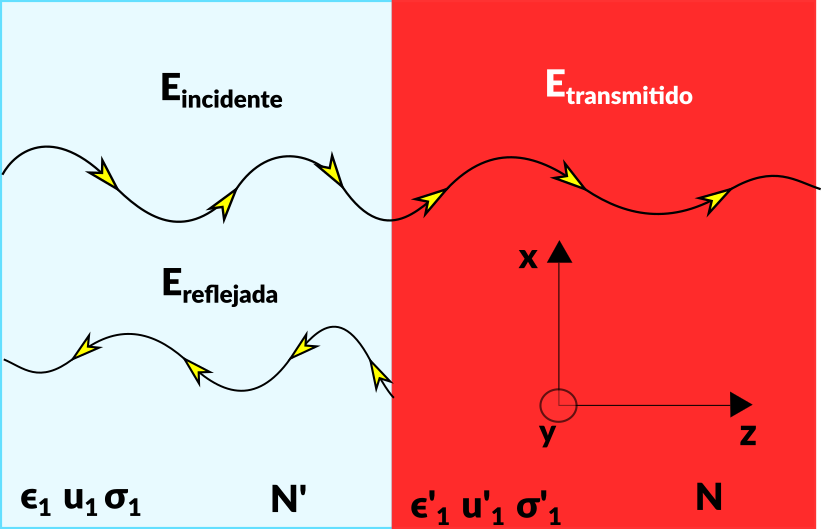
\includegraphics[width=420px, height=180px]{reflectividadNormal.png}\label{reflectividadFigura}\\
\begin{center}
Figura \ref{reflectividadFigura}. Reflectividad a incidencia normal.
\end{center}

Dentro del solido la onda sera atenuada. Asumiremos que el solido es lo suficientemente delgado  para ignorar reflexiones internas \cite{SolidStatePhysics}. Ahora la siguiente pregunta sera como cambia la propagación de la onda electromagnética cuando pasa de estar en un medio de espacio vacío a un medio material. Consideremos la propagación de un plano de onda electromagnético que viene desde el vacío ($\varepsilon^{'}_{1}=\mu_{1}^{'}=1,\sigma_{1}^{'}=0$) y pasa a través de un medio de material con $\mu_{1}=1$ y $\varepsilon_{1}$, $\sigma_{1}$ finitos.

La superficie se encuentra en el plano XY, mientras que  el eje Z  positivo esta en la dirección normal hacia la superficie descrito por el vector unitario $n_{s}$. Por lo que la dirección de propagación de la onda estaría en el plano XZ como se muestra en la figura.

El campo eléctrico y magnético transmitido dentro del solido esta dado por:
\begin{equation}\label{Ei1}
\vec{E}_{xt}(z,t)=E_{0t}e^{i(\vec{q}_{i}\cdot z -wt)}
\end{equation}
\begin{equation}\label{Ei2}
\vec{H}_{yt}(z,t)=E_{0t}e^{i(\vec{q}_{i}\cdot z -wt)}
\end{equation}
Con el vector de onda dado por $\vec{q}_{i}=\frac{w}{c}\hat{N}$
Por otro lado en el espacio vacío tenemos una onda incidente y una reflejada dadas por:

\begin{equation}\label{Et1}
\vec{E}_{xi}(z,t)=E_{i}e^{i(\frac{wz}{c}-wt)}+E_{r}e^{i(\frac{-wz}{c}-wt)}
\end{equation}
\begin{equation}\label{Et2}
\vec{H}_{yi}(z,t)=E_{i}e^{i(\frac{wz}{c}-wt)}-E_{r}e^{i(\frac{-wz}{c}-wt)}
\end{equation}
En la interfaz de los dos medios las componente de $E_{xi}$ y $H_{yi}$ debe ser continuas a través de la superficie, esto requiere que se cumpla:

\begin{equation}\label{Ecuacioncondicion}
E_{t}=E_{i}+E_{r}
\end{equation}
\begin{equation}
H_{t}=H_{i}-H_{r}
\end{equation}
De la ecuación de Maxwell(ley de Faraday) \ref{1.1} se tiene:
\begin{equation}
\nabla\times \vec{E}(r,t)=-\frac{1}{c}\frac{\partial\vec{H}(r,t)}{\partial t}=\frac{iw}{c}\vec{H}(r,t)
\end{equation}

Que en nuestro caso resulta:

\begin{equation}\label{continuidad1}
\frac{\partial \vec{E}(r,t)_{x}}{\partial z}=\frac{iw}{c}\vec{H}(r,t)_{y}
\end{equation}
Combinando la ecuación \ref{continuidad1} con \ref{Ei1} y \ref{Et2} se llega a:

\begin{equation}
E_{t}\vec{q}_{t}=E_{i}\frac{w}{c}-E_{r}\frac{w}{c}=E_{0}\frac{w}{c}\hat{N}
\end{equation}
O también lo que es lo mismo:

\begin{equation}\label{condicionN}
E_{i}-E_{r}=E_{t}\hat{N}
\end{equation}
Combinando la ecuación \ref{condicionN} y \ref{Ecuacioncondicion} se obtiene el coeficiente de reflexión complejo como nueva función de respuesta ya que relaciona la radiación reflejada e incidente:

\begin{equation}
\hat{r}=\frac{E_{r}}{E_{i}}=\frac{1-\hat{N}}{1+\hat{N}}=|\hat{r}|e^{\{i\phi_{r}\}}=\sqrt{\frac{I_{r}}{I_{i}}}e^{\{i\phi_{r}\}}=\sqrt{R}e^{\{i\phi_{r}\}}
\end{equation}

Durante el experimento usualmente la reflectancia R es medida  y la información del cambio de fase de la onda se pierde ya que se esta midiendo el modulo de $|\hat{r}|=R$.
\begin{equation}
R=\frac{|E_{r}|^{2}}{|E_{i}|^{2}}=|\hat{r}|^{2}=|\frac{1-\hat{N}}{1+\hat{N}}|^{2}=\frac{(1-n)^{2}+k^{2}}{(1+n)^{2}+k^{2}}
\end{equation}
El cambio de fase de la onda estará dada por:

\begin{equation}
tan\phi_{r}=\frac{-2k}{1-n^{2}-k^{2}}
\end{equation}

La conductividad compleja y la función dieléctrica pueden definirse  en términos de la reflectancia y el cambio de fase como:

\begin{equation}
\sigma_{1}(w)=\frac{w}{4\pi}\varepsilon_{2}(w)=\frac{w}{4\pi}\frac{4\sqrt{R(w)}[1-R(w)]sin\phi_{r}}{[1+R(w)-2\sqrt{R(w)cos\phi_{r}}]^{2}}
\end{equation}
\begin{equation}
\sigma_{2}(w)=\frac{w}{4\pi}[1-\varepsilon_{1}(w)]=\frac{w}{4\pi}(1-\frac{[1-R(w)]^{2}-4R(w)sin^{2}\phi_{r}}{[1+R(w)-2\sqrt{R(w)}cos\phi_{r}]^{2}})
\end{equation}

La trasmisión $\hat{t}$ también puede ser determinado para una onda electromagnética que atraviesa la  superficie:
\begin{equation}
\hat{t}=\frac{E_{t}}{E_{i}}=\frac{2N^{'}}{N+N^{'}}=|\hat{t}|e^{i\phi_{t}}
\end{equation}
Y el cambio de fase:
\begin{equation}
\phi_{t}=arctan\{\frac{n-k}{n+k}\}
\end{equation}
Este es cambio de fase entre la onda incidente y la onda transmitida. Por lo que se puede definir la tramitancia como:
\begin{equation}
T=\frac{I_{t}}{I_{i}}=\sqrt{\varepsilon_{1}}\frac{|E_{t}|^{2}}{|E_{i}|^{2}}=\sqrt{\varepsilon_{1}}|\hat{t}|^{2}=\frac{4n}{(n+1)^{2}+k^{2}}=1-R
\end{equation}


El conocimiento del índice de refracción complejo ($N$) permite calcular R y por lo tanto T. La transmitividad en un medio absorbente de grosor l esta dado por \cite{MarkFox}:
\begin{equation}
T=(1-R_{1})e^{-\alpha l}(1-R_{2})
\end{equation}
Donde $R_{1}$ y $R_{2}$ son las reflectividades en el frente de superficie y la reflectividad al final del material. Si el frente del material y el fondo del material poseen la misma reflectividad, como es usual, entonces la ecuación anterior se puede simplificar \cite{MarkFox}:
\begin{equation}
T=(1-R)^{2}e^{-\alpha l}
\end{equation}
En materiales transparentes como los vidrios en el espectro de luz visible el coeficiente de absorción es muy pequeño. Por lo que en este rango se pueden despreciar $k$ y $\varepsilon_{2}$ y por lo tanto el índice de refracción complejo y la función dieléctrica son tomados como números reales. Esta es la razón por la que en las tablas de propiedades generalmente solo las partes reales de la función dieléctrica y el índice de refracción complejo son mostrados \cite{MarkFox}.

\section{Relaciones Kramers Kronig}
Los diferentes parámetros ópticos y constantes ópticas describen la respuesta del medio aplicando radiación electromagnética dentro del marco de la teoría de respuesta lineal, la dependencia de la frecuencia de la función de respuesta es llamada dispersión. La constante dieléctrica compleja $\varepsilon$ y la conductividad $\sigma$ pueden ser consideradas como las principales funciones de respuesta del material, describiendo la polarización eléctrica y corrientes inducidas en respuesta a campos eléctricos. El cambio de la onda electromagnética en el material también puede darse en términos del índice de refracción complejo $\hat{N}$ y en términos de la impedancia $Z_{s}$ , los cuales también son funciones de respuesta complejas. Por lo que siempre se trata con funciones de respuesta complejas que describen la respuesta del sistema a estímulos, por lo que siempre habrá disipación y cambios de fase \cite{electrodynamics}. 

Consideraciones generales que involucran causalidad, son usados para derivar importantes relaciones entre la parte real y imagina de funciones de respuesta complejas. Estas fueron dadas por Kramers y Kronig y juegan un papel muy importante mas allá de la teoría de funciones de respuesta. Estas relaciones tienen también una gran importancia practica ya que permiten la evaluaciones de las componentes de la función dieléctrica compleja  o conductividad, cuando solo un parámetro óptico como el poder reflejado, transmitido o absorbido es medido \cite{electrodynamics}.

Para derivar estas relaciones, asumamos una respuesta lineal a una perturbación externa dada de la forma \cite{electrodynamics}:

\begin{equation}\label{1.36}
\hat{X}=\int\int_{-\infty}^{\infty}\hat{G}(r,r^{'};t,t^{'})\hat{f}(r^{'},t^{'})dr^{'}dt^{'}
\end{equation}

Esto describe la respuesta $\hat{X}$ del sistema en el tiempo t y posición r a un estimulo $\hat{f}$ en el tiempo $t^{'}$ y posición $r^{'}$. La función $\hat{G}(r,r^{'};t,t^{'})$ es llamada función de respuesta , y puede ser la conductividad, la constante dieléctrica, la susceptibilidad, o otra constante óptica como el índice de refracción. En nuestro caso  el estimulo sera un onda electromagnética, también asumiremos que el medio es isotropico y homogéneo por lo que despreciaremos la dependencia espacial, así $\hat{G}$ es un escalar. Y ya que el origen de la escala del tiempo no tiene importancia física, entonces $G(t,t^{'})$ es una función de la diferencia de los argumentos $t-t^{'}$ , así lo que ocurre en un lugar particular depende solo de los campos existentes en el lugar. En lo que sigue despreciaremos la dependencia espacial de la perturbación externa, y nos restringiremos a una aproximación local. Entonces la respuesta en una posición particular r depende solo del campo en el cual existe en un lugar particular descrito por la función delta ($\delta(x)=1$ si $x=0$). 

\begin{equation}\label{1.37}
\hat{G}(r,r^{'};t,t^{'})=\delta(r-r^{'})\hat{G}(t-t^{'})
\end{equation}

Con las condiciones tomadas la ecuación \ref{1.36} se convierte en:
\begin{equation}\label{1.38}
\hat{X}(t)=\int_{-\infty}^{\infty}\hat{G}(t-t^{'})\hat{f}(t^{'})dt^{'}
\end{equation}

Si el sistema es causal entonces  para $t<t^{'}$:
\begin{equation}\label{1.39}
\hat{G}(t-t^{'})=0 
\end{equation}
Lo cual básicamente significa que no habrá respuesta antes del estimulo y podemos escribir $\int_{-\infty}^{\infty}dt^{'} $ a $\int_{-\infty}^{t}dt^{'}$.

Es conveniente tratar con cantidades en el dominio de frecuencias. En el espacio de Fourier se pueden definir como \cite{OpticalTechniques}:

\begin{equation}\label{1.40}
\hat{f}(w)=\int \hat{f}(t)exp\{iwt\}dt
\end{equation}

\begin{equation}\label{1.41}
\hat{X}(w)=\int \hat{X}(t)exp\{iwt\}dt
\end{equation}

\begin{equation}\label{1.42}
\hat{G}(w)=\int \hat{G}(t-t^{'})exp\{iw(t-t^{'})\}dt
\end{equation}
Por lo que la respuesta se puede escribir colocando \ref{1.38} en \ref{1.41} llevando a la convolución:
\begin{equation}\label{1.43}
\hat{X}(w)=\int dt exp\{iwt\}[\int \hat{G}(t-t^{'})\hat{f}(t^{'})dt^{'}]
\end{equation}
\begin{center}
$
=\displaystyle\int dt^{'}\hat{f}(t^{'})exp\{iwt^{'}\}[\int \hat{G}(t-t^{'})exp\{iw(t-t^{'})\}dt]
$
\end{center}
\begin{center}
$
=\hat{G}(w)\hat{f}(w)
$
\end{center}

Así en el dominio de frecuencia la respuesta $X(w)$ es igual a la multiplicación de un estimulo monocromático $f(w)$ por un numero $G(w)$, llamado susceptibilidad \cite{OpticalTechniques}. Generalmente $\hat{G}$ es una cantidad compleja, con la componente real describiendo la amplitud de la respuesta y la parte imaginaria refleja la diferencia de fase entre el estimulo y la respuesta. Por razones matemáticas, se asume que la frecuencia que aparece en las ecuaciones anteriores es compleja, $\hat{w}=w_{1}-iw_{2}$, entonces de la ecuación \ref{1.42} sera:
\begin{equation}
\hat{G}(\hat{w})=\int \hat{G}(t-t^{'})exp\{iw_{1}(t-t^{'})\} exp\{-w_{2}(t-t^{'})\} dt
\end{equation}
Esta integral puede ser evaluada usando el teorema de la integral de Cauchy. El factor $exp[-w_{2}(t-t^{'})]$ esta 
limitado por la parte superior del plano complejo para $t-t^{'}>0$ y abajo de la mitad del plano complejo para $t-t^{'}<0$. El requerimiento de casusalidad requiere que sea evaluado sobre la mitad superior del plano complejo \cite{electrodynamics}.

Si consideramos el contorno de un semicirculo cerrado como muestra la figura[x] con un pequeño bulto al rededor de la frecuencia w, del teorema de Cauchy se puede escribir:

\begin{equation}
\hat{G}(w)=\frac{1}{i\pi}\wp\oint \frac{\hat{G}(\hat{w}^{'})}{\hat{w}^{'}-\hat{w}_{0}}d\hat{w}^{'}=0
\end{equation}

Ahora consideremos el caso limite cuando el radio del semicirculo tiende a infinito mientras que el radio del pequeño semicirculo al rededor de $w_{0}$ se aproxima a cero. Mientras que la integral sobre el largo el semicirculo desaparece como $\hat{G}(\hat{w})\rightarrow 0$ cuando $\hat{w}^{'}\rightarrow\infty$, la integral sobre el pequeño semicirculo de radio $\eta$ puede ser evaluado usando $\hat{w}^{'}=\hat{w}_{0}-\eta exp\{i\phi \}$, esta relación es aveces llamada identidad de Dirac: 

\begin{equation}
\lim_{n\rightarrow 0}\frac{1}{x \pm i\eta}=\wp\{\frac{1}{x}\} 	\mp i\pi \delta(x)
\end{equation}
Por lo que obtenemos:
\begin{equation}
\lim_{n\rightarrow 0}\oint \frac{\hat{G}(\hat{w}^{'})}{\hat{w}^{'}-\hat{w}_{0}}d\hat{w}^{'}=-i\pi \hat{G}(\hat{w}_{0})
\end{equation}
Esta integral a lo largo del eje real de frecuencia da el principal valor de P. Sin embargo:

\begin{equation}
\hat{G}(w)=\frac{1}{i\pi}\wp\int_{-\infty}^{\infty}\frac{\hat{G}(w^{'})}{w^{'}-w}dw^{'}
\end{equation}
Donde hemos omitido el índice $w_{0}$. En la manera usual, la función de respuesta compleja $\hat{G}(w)$ puede estar escrita en términos de la parte real y imagina como $\hat{G}(w)=G_{1}(w)+iG_{2}$ llevando a la siguientes relaciones de dispersión entre las partes reales e imaginaria de la función de respuesta:

\begin{equation}
G_{1}(w)=\frac{1}{\pi}P\int_{-\infty}^{\infty}\frac{G_{2}(w^{'})}{w^{'}-w}dw^{'}
\end{equation}

\begin{equation}\label{g}
G_{2}(w)=-\frac{1}{\pi}P\int_{-\infty}^{\infty}\frac{G_{1}(w^{'})}{w^{'}-w}dw^{'}
\end{equation}
Notemos que \ref{g} nos dice que si tenemos determinado $G_{1}(w)$ sobre todas las frecuencias entonces podemos encontrar $G_{2}(w)$. Así se puede observar que la parte real e imaginaria no son independientes pero están relacionada.

Usando estas relaciones podemos derivar varias expresiones conectando la parte real e imaginaria de diferentes parámetros ópticos y funciones de respuestas mencionados anteriormente. Para Aplicar estas relaciones a la constante dieléctrica compleja, se tiene la polarización P en respuesta a un campo eléctrico E aplicado lleva a un desplazamiento D dado por la ecuación  \ref{1.5} :
\begin{equation}
4\pi P(w)=[\varepsilon_{1}(w)-1]E(w)
\end{equation}
Consecuentemente $\varepsilon_{1}(w)-1$ es la función de respuesta apropiada:
\begin{equation}
\varepsilon_{1}-1=\frac{2}{\pi}P\int_{0}^{\infty}\frac{w^{'}\varepsilon_{2}(w^{'})}{(w^{'})^{2}-w^{2}}dw^{'}
\end{equation}
Para la parte imaginaria:
\begin{equation}
\varepsilon_{2}=-\frac{2w}{\pi}P\int_{0}^{\infty}\frac{\varepsilon_{1}(w^{'})}{(w^{'})^{2}-w^{2}}dw^{'}+\frac{4\pi\sigma
_{dc}}{w}
\end{equation}
Con $\sigma_{dc}$ dado por:
\begin{equation}
\sigma_{dc}=\sigma_{1}(0)=\frac{1}{2\pi^{2}}\int_{0}^{\infty}[1-\varepsilon_{1}(w^{'})]dw^{'}
\end{equation}
También puede ser usada para otras constantes ópticas que puede llamarse funciones de respuesta como el índice de refracción compleja $N(w)=n(w)+ik(w)$ y están dadas por:
\begin{equation}
n(w)-1=\frac{2}{\pi}\wp\int_{0}^{\infty}\frac{w^{'}k(w^{'})}{(w^{'})^{2}-w^{2}}dw^{'}
\end{equation}
\begin{equation}
k(w)=\frac{-2}{\pi w}\wp\int_{0}^{\infty}\frac{(w^{'})^{2}[n(w^{'}-1)]}{(w^{'})^{2}-w^{2}}dw^{'}
\end{equation}
Podemos escribir las relaciones de dispersión entre la amplitud $\sqrt{R}=|\hat{r}|$ y el cambio de fase $\phi_{r} $ de la onda reflejada fuera de la superficie de una muestra. Escribiendo $Ln \hat{r}(w)=ln|\hat{r}(w)|+i\phi_{r}(w)$ las relaciones serán:
\begin{equation}
ln|\hat{r}(w)|=\frac{1}{\pi}\wp\int_{-\infty}^{\infty}\frac{\phi_{r}(w^{'})}{w^{'}-w}dw^{'}
\end{equation}
\begin{equation}
\phi_{r}(w)=-\frac{1}{\pi}\wp\int_{-\infty}^{\infty}\frac{ln|\hat{r}(w^{'})|}{w^{'}-w}dw^{'}
\end{equation}
\section{Materiales en Estado Solido}
Ahora se pasara al estudio de las propiedades ópticas de diferentes tipos de materiales en estado solido. Los materiales pueden clasificarse en cinco categorías generales:
\begin{itemize}
\item Aislantes Cristalinos y Semiconductores.
\item Vidrios.
\item Metales.
\item Materiales moleculares
\item Vidrios dopados y aislantes.
\end{itemize}
Por lo que describiremos cada una de esta clasificaciones, esto como una introducción a las propiedades ópticas físicas que se trataran mas adelante.

\subsection{Aislantes Cristalinos y Semiconductores}

En la figura \ref{zafiro} se muestra el espectro de transmisión de un cristal de zafiro($Al_{2}O_{3}$) desde frecuencias del infrarrojo hasta el ultravioleta. El espectro del zafiro muestra las principales características en todos los aislantes, pero por supuesto varían en detalle de material a material\cite{SolidStatePhysics}. 
\begin{center}
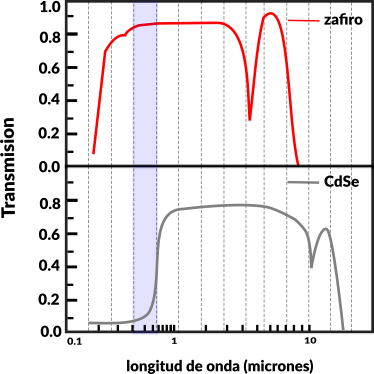
\includegraphics[width=300px, height=300px]{transmision.png}\label{zafiro}\\

Figura \ref{zafiro}.a) Espectro de transmisión de una muestra de zafiro($Al_{2}O_{3}$) de 3mm de grosor. b) espectro de transmision de un cristal de $CdSe$ de grosor 1.67mm \cite{MarkFox}.
\end{center}



Las principales propiedades ópticas pueden resumirse en las siguientes:
\begin{itemize}
\item El zafiro tiene una alta transmisión en el rango de longitudes de onda desde 0.2 a 0.6$\mu m$, esto define el rango de transparencia del cristal. La regios de transparencia incluye todo rango del espectro visible eso explica porque el zafiro es incoloro y transparente para el ojo humano.
\item dentro del rango de transparencia el coeficiente de absorción es muy pequeño, y el índice de refracción complejo puede tomarse real sin parte imaginaria. El valor del índice de refracción es aproximadamente constante y es igual a 1.77 en el zafiro.
\item La profunda caída de la transmisión en el infrarrojo cerca de 3$\mu m$ y para $\lambda >6\mu m$ es causada por vibraciones que absorben la radiación. Estas excitaciones vibracionales de la red de un cristal son llamadas modos fononicos, y así la absorción vibracional en un solido es llamada absorción fononica o absorción de la red. El mecanismo de absorción se describirá mas adelante.
\item Las caídas de transmisión en el rango ultravioleta para $\lambda<0.2\mu m$ es debido a la absorción fundamental por electrones de bandas. Las longitudes de onda que ocurren para las absorciones están determinadas por las bandas electrónicas del aislante, la explicación de este proceso se trata mas adelante.
\end{itemize}

Seguramente la característica mas obvia de las propiedades ópticas de los aislantes, es  que tienden son incoloros y transparentes en el espectro visible. Si tienden a tener color es debido a la presencia de impurezas. Los aislantes absorben fuertemente radiación ultravioleta y infrarroja pero esto escondido del ojo humano. Las regiones de transparencia entre el infrarrojo y ultravioleta es particularmente útil para hacer lentes \cite{SolidStatePhysics}.

El ejemplo de la figura \ref{zafiro} b) muestra el espectro de transmisión de un semiconductor compuesto II-VI sobre el mismo rango de frecuencias que el zafiro. Al igual que en el zafiro, tiene un rango de transparencia que esta limitados por la absorción eléctrica a cortas longitudes de onda y absorciones de red a longitudes mayores. La máxima transmisión es al rededor del $60\%$ ,  el rango de transparencia se mantiene fuera del espectro visible. Por la tanto en el cristal no se transmitirá luz visible por lo que le da una color metálico oscura \cite{MarkFox}.

\subsection{Vidrios}
Los vidrios son muy importantes en óptica de materiales. Son usada por siglos en prismas y lentes para instrumentos ópticos. En tiempos mas recientes se han encontrado nuevas aplicaciones en tecnología de fibra óptica. La mayoría de vidrios se hacen fusionando arena($SiO_{2}$) con otros químicos. El silicio puro es un aislante y muestra todas las características que se destacan de los aislantes discutidas con anterioridad. Es transparente en el espectro visible pero absorbe ultravioleta debido a transiciones electrónicas de las moléculas de silicio, y en el rango infrarrojo debido a vibraciones de red. Este material es extensamente utilizado en la industria óptica, ya que es el material principal del que están hechas las fibras ópticas, ha sido refinado hasta tal punto que el coeficiente de extinción es tan pequeño que la luz puede viajar muchos kilómetros antes de ser atenuada y el coeficiente de refracción varia menos del $1\%$ en el espectro visible debido a la dispersión. La dispersión sera mayor para frecuencias cerca de absorciones fundamentales.

Químicos son comúnmente agregados al silicio durante el proceso de fusión para producir otros tipos de vidrios. La presencia de estos aditivos alteran el índice de refracción y el rango de transmisión.

\subsection{Metales}
La característica mas resaltante de los metales es que son brillantes. Debido a esto metales como la plata y el aluminio han sido usando como espejos durante siglos. Su brillo es consecuencia de sus altos coeficientes de reflexión causada por la interacción de la luz con los  electrones libres presentes en el metal.



\begin{center}
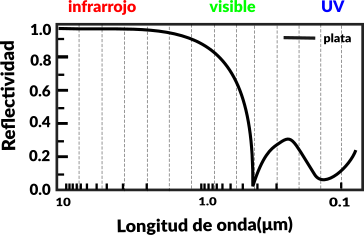
\includegraphics[width=300px, height=230px]{plata.png}\label{silver}\\

Figura \ref{silver}. Reflectividad de la plata desde el infrarrojo hasta el ultravioleta \cite{MarkFox}.
\end{center}

La figura \ref{silver} muestra la reflectividad de la plata desde la región del espectro infrarrojo hasta el ultravioleta. Se puede observar que la reflectividad es casi del $100\%$ en rango infrarrojo, y se mantiene sobre el $80\%$ en la región del espectro visible. En la región del espectro ultravioleta decae rápidamente, esto es una característica común en todos los metales. Existe una fuerte reflexión para todas las frecuencias por debajo de una frecuencia de corte llamada frecuencia del plasma. Así los metales reflejan longitudes de onda infrarrojas y visibles, pero transmiten longitudes de onda ultravioleta. Los colores observados en los metales son causados por transiciones entre las bandas electrónicas que ocurren además de los efectos causados por la reflexión.
\subsection{Materiales Moleculares}
El termino "material molecular" en principio cubre el estado solido de cualquier molécula. Sin embargo estados cristales de molecular inorgánicas como el $NaCl$ o $GaAs$ se clasifican aislantes o semiconductores, mientras que molecular orgánicas simples como el metano $CH_{4}$ tienden a ser gases o líquidos a temperatura ambiente. Enfocaremos la atención a moléculas orgánicas grandes.
Algunos componentes orgánicos forman cristales en la fase condensada, pero otros pueden ser amorfos. Los solidos se mantienen unidos debido a interacciones van der Waals débiles entre moléculas, y así mismos se encuentran atados a fuertes enlaces covalentes. Las propiedades ópticas de los solidos se aplican a moléculas individuales.

Los componentes orgánicos generalmente se clasifican en sistemas saturados o conjugados. Esta clasificación depende del tipo de enlaces en la molécula.

En componentes saturados, los electrones de valencia se incorporan en fuertes bandas localizadas entre átomos vecinos. Esto significa que los electrones de banda se encuentran altamente concentrados en las bandas, y solo responden a altas frecuencias del espectro ultravioleta. 

Los componentes saturados en contraste tienen propiedades ópticas mas interesantes. Los electrones del estados atómicos p de átomos de carbono forman orbitales delocalizados llamados orbitales $\pi$ los cuales se esparcen a través de la molécula entera. El ejemplo están de una molécula conjugada es el benceno $C_{6}H_{6}$, en la cual los electrones $\pi$ forman un anillo orbital sobre y por debajo del plano de los átomos de carbono e hidrógeno. Otros ejemplos incluyen hidrocarburos aromáticos, molecular dye, y polímeros conjugados.

Los electrones $\pi$ están menos atadas a las bandas que los electrones en moléculas saturada, y son opticamente activa a bajas frecuencias. En el benceno la absorción fundamental se da en el ultravioleta a 260nm, pero con otras moléculas la energía de transición cambio por debajo de frecuencias visibles. Esto entonces es de gran interés para dispositivos que emiten luz.

Por ejemplo la figura \ref{polifluoreno} muestra el espectro de absorción del polímero tecnologicamente importante basado en polifluoreno llamado F8. Los datos en la figura muestra que el polímero es transparente en la mayor parte del espectro visible, pero absorbe altamente el espectro ultravioleta. La banda de absorción que aparece en 380nm es causada por transiciones vibraciones electrónicas al primer estado excitado de la molécula. Esta banda se extiende hasta la región del espectro azul y le da al material un color amarillo pálido.

\begin{center}
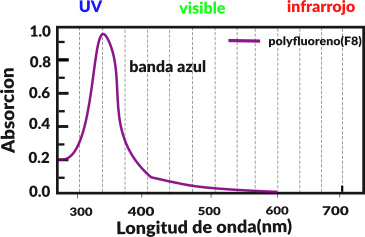
\includegraphics[width=300px, height=230px]{polifluoreno.png}\label{polifluoreno}\\

Figura \ref{polifluoreno}. Espectro de absorción de el polifluoreno polímero F8 \cite{MarkFox}.
\end{center}

\subsection{Vidrios dopados y aislantes}
Ya se menciono que los aislantes que tienen a tener color están hechos por agregar algún semiconductor al silicio en el proceso de fusión. Este es un ejemplo de como los materiales incoloros tales como el silicio pueden tomar nuevas propiedades controlando el dopamiento con sustancias ópticas activas.

El color de un vidrio filtro del color puede ser controlado de dos diferentes formas:
\begin{itemize}
\item La forma mas obvia es variando la composición del dopante. Por ejemplo el vidrió puede ser dopado con el semiconductor $Cd_{x}Zn_{I-x}Se$ durante el proceso de fusión, con el valor x determinado por la relación $ZnSe:CdSe$ de la mezcla original. El ancho de banda de la aleación puede ser colocado en la región del espectro visible variando x, y esto determina la transmisión  de la longitud de onda  para el filtro.
\item El tamaño del semiconductor cristales dentro del vidrio puede ser muy pequeño, y esto puede tener un efecto en el color producido. Normalmente las propiedades ópticas de un material  son independiente del tamaño del cristal, pero si lo es para el caso de dimensiones comparables con las longitudes de onda del electrón. El tamaño del efecto cuántico incrementa la energía de los electrones y por lo tanto cambia el ancho de banda a altas energías.
\end{itemize}

El principio de dopamiento de átomos opticamente activos es empleado extensamente en los cristales usados para láseres. Un típico ejemplo es el rubí.   Los rubíes resultan de dopar iones de $Cr^{3+}$ en $Al_{2}O_{3}$(zafiro). En cristales naturales, los iones están presentes como impurezas, pero en cristales sintéticos, los dopantes son deliberadamente introducidos en cantidades controladas durante el proceso de crecimiento del cristal.
La figura \ref{zarubi} compara el espectro de transmisión del rubí sintético ($Al_{2}O_{3}$ con $0.05\%$ $Cr^{3+}$) con el zafiro sintético ($Al_{2}O_{3}$ puro). Se puede ver que la presencia de los iones de chromonium producen dos fuertes bandas de absorción. una en el espectro azul, y otra en la región del amarillo/verde. Estas dos bandas de absorción dan a los rubíes su característico color rojo. Otra diferencia obvia entre las dos curvas es que la transmisión del rubí es menor. Esto es causado en parte por el aumento de la dispersión de la luz por las impurezas del cristal. 

\begin{center}
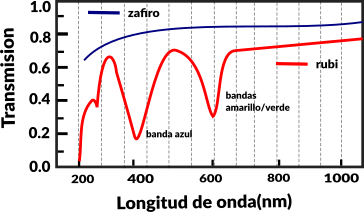
\includegraphics[width=330px, height=230px]{rubi.png}\label{zarubi}\\

Figura \ref{zarubi}. Espectro de transmisión del rubí comparado con el zafiro. El grosor de las muestras es de 6.1 mm y 3.0mm respectivamente \cite{MarkFox}.
\end{center}



\section{Características ópticas físicas en el estado solido}
En la sección anterior se dio una introducción a las propiedades ópticas de diferentes clases de materiales en estado solido. Es natural preguntarse si estas propiedades son exclusivas del estado solido. En otras palabras como las propiedades ópticas son diferentes entre aquellos materiales que están constituidos por átomos o moléculas. Esta pregunta es esencialmente la misma que preguntar cual es la diferencia entre el estado solido, atómico y molecular.

La respuesta depende claramente del tipo de material que estemos considerando. En algunos materiales habrán un rango entero de nuevos efectos asociados con el estado, mientras que en otros, las diferencias no son muy grandes.
Los materiales moleculares son un ejemplo del segundo tipo. Podemos esperar que el espectro de absorción de una capa de solido es equivalente a una solución del material.  Esto pasa porque las fuerzas entre las moléculas en la fase condensada son débiles comparada con la fuerzas dentro de la molécula en si misma.  
Con muchos otros materiales sin embargo habrá diferencias sustanciales entre la fase condensada y la fase liquida o gaseosa. Por lo que trataremos cinco aspecto que hacen la física de estado solido interesante y diferente \cite{MarkFox}.
\subsection{Simetría Cristalina}
La mayoría de los materiales que se estudian son cristales. Los cristales tienen un alto rango orden translacional y pueden ser categorizados en 32 clases de acuerdo a su simetría. La simetría dependerá de las operaciones que hacen que el cristal sea invariante. Un ejemplo son las rotaciones sobre un eje en particular. Algunos cristales como los cúbicos poseen un alto grado de simetría.
El enlace entre las cantidades medibles y el grupo de simetría esta dado por el principio de Neumann el cual establece que cualquier propiedad física macroscópica debe tener la estructura cristalina del cristal. Por ejemplo si un cristal tiene la misma simetría sobre sus cuatro ejes de rotación entonces el mismo resultado se encontrara en cualquier experimento que se haga sobre los cuatro rotaciones.

Es interesante comparar las propiedades del cristal con las propiedades de los átomos individuales de los cuales esta formado. En un gas los átomos no tienen orden translacional. Sin embargo se espera que encontrar efectos en el estado solido que reflejen la simetría translacional del cristal. La formación de bandas electrónicas y estados de-localizados son ejemplos de esto. Al mismo tiempo el grupo de simetría del cristal es menor que el átomo individual. El cual posee la mas alta simetría posible debido a invariancia esférica.
Sin embargo se espera encontrar otros efectos en el estado solidos relacionados la disminución de la simetría. Dos ejemplos de estos se discutirá brevemente la anisótropo óptica y el alzamiento de degeneraciones \cite{MarkFox}.

Un cristal se dice anisotropico si sus propiedades no son las mismas en todas las direcciones. La anisotropia es solo encontrada en el estado solido porque en estado liquido y gaseoso no hay direcciones preferidas. El grado de anisotropia encontrada en cristales depende fuertemente del grupo de simetría al cual pertenece.

En redes cubicas simples por ejemplo las propiedades deben ser las mismas a lo largo de las direcciones x, y, z porque son físicamente indistinguibles. Por otro lado en un cristal uniaxial, las propiedades a lo largo del eje óptico serán distintas a las otras direcciones. La anisotropia óptica se manifiesta por la propiedad de birrefringencia.

El alzamiento de degeneraciones por reducción de la simetría es un efecto conocido en física atómica. Los átomos libres tienen simetría esférica por lo que no tienen direcciones preferidas. La simetría se puede romper si aplicamos un campo eléctrico o magnético externo lo cual crea una dirección de preferencia a lo largo de la dirección del campo. Esto puede llevar al levantamiento de ciertos niveles de degeneración que son presentes en átomos libres. El efecto Zeeman por ejemplo, describe la separación de los niveles de degeneración magnéticos cuando un campo magnético es aplicado. Si el mismo átomo es introducido en un cristal, este se encontrara en un ambiente con un grupo de simetría determinado por la red cristalina. La simetría sera menor que cuando el átomo estaba solo y se alzaran nuevos niveles de degeneración \cite{MarkFox}.

En la figura \ref{zeeman} este punto es ilustrado, donde se muestra como los niveles magnéticos de átomos libres pueden ser divididos por el efecto del campo que produce el cristal de la misma manera que lo hace el efecto Zeeman. La división es causada por la interacción de los orbitales de los átomos dentro de campos eléctricos en el cristal. Los detalles no serán tratados aquí, el punto importante es que las divisiones son determinadas por la clase de simetría del cristal. Las transiciones ópticas entre estos niveles del campo del cristal frecuentemente ocurren en la región del espectro visible, y causa que los materiales tengan interesantes propiedades que no son encontrados en átomos individuales. Vale la pena señalar que muchos materiales solidos importantes no poseen simetría translacional. EL vidrio es un ejemplo, otros ejemplos incluyen películas moleculares tales como polímeros emisores de luz pulverizados sobre substratos y silicio amorfo.  Las propiedades ópticas de estos materiales pueden ser muy similares a las propiedades de los átomos o moléculas individuales que están constituidos \cite{MarkFox}.

\begin{center}
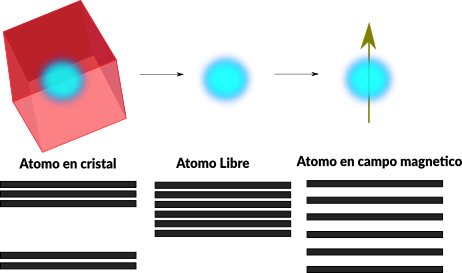
\includegraphics[width=330px, height=230px]{degeneracion.png}\label{zeeman}\\

Figura \ref{zeeman}. División de los niveles magnéticos de un átomo libre por el efecto del campo del cristal. En los tres átomos, los niveles magnéticos son degenerados. Debemos aplicar un campo magnético para dividir los niveles, sin embargo los niveles puede ser divididos sin aplicar un campo magnético externo cuando se encuentra dentro del cristal.
\end{center}



\subsection{Bandas Electrónicas}
Los átomos en un solido están agrupados muy cerca uno del otro, con la separación interactomica aproximadamente igual al tamaño de los átomos. Por lo tanto los orbitales mas externos se sobreponen y interactúan fuertemente uno con el otro. La ampliación de niveles discretos de átomos libres en bandas, es ilustrado en la figura \ref{bandaselectronicas}.
 

\begin{center}
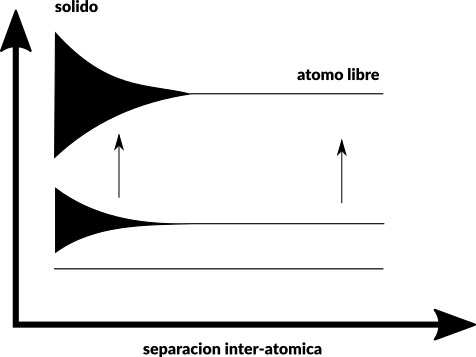
\includegraphics[width=300px, height=230px]{separacion.png}\label{bandaselectronicas}\\

Figura \ref{bandaselectronicas}. Diagrama esquemático de la formación de bandas electrónicas en un solido desde la condensación de los átomos libres. Como los átomos se encuentran tan cercanos el uno del otro que sus orbitales mas externos se sobreponen, esto produce la formación de bandas.
\end{center}

 
 
El estado del electrón dentro de la banda esta de-localizado y posee la invariancia translacional del cristal. Por el teorema de Bloch que establece que las funciones de onda pueden ser escritas de la forma:

\begin{equation}
\phi_{k}(r)=\mu_{k}(r)exp(ek\cdot r)
\end{equation}

Donde $\mu_{r}(r)$ es una función que tiene la periodicidad de la red. En los estados Bloch descritos por la ecuación anterior son modulados por ondas planas. Cada banda electrónica tiene una función $\mu_{r}(r)$ asociada que mantiene la información de algún estado atómico del cual surge la banda. 

Las transiciones ópticas pueden ocurrir entre bandas electrónicas si lo permiten las reglas de selección. Esta absorción interbandas es posible sobre un rango continuo  del photon determinado por la energía mas baja y mas alta de los limites de las bandas. Esto contrasta con el espectro de absorción de átomos libres, ya que estos consisten de lineas discretas. La observación de bandas de absorción mas que lineas discretas es una de las características destacadas del estado solido. La fuerza de absorción es usualmente muy alta por la alta densidad de átomos absorbentes en el solido.

\subsection{Bandas Vibracionales}

El estado electrónico de los átomos o moléculas en un solido pueden estar fuertemente ligados a los modos vibracionales del cristal a través de la interacción vibronica. Un ejemplo típico donde este efecto ocurre es en el aislante cristalino dopado \ref{zarubi}. El ligamento vibronico amplia los estados electrónicos discretos de las lineas de absorción y emisión de los átomos dentro de las bandas continuas. 

Es importante darse cuenta que la razón de la formación de las bandas vibronicas es diferentes a de las bandas electrónicas consideradas anteriormente. 

En el caso de las bandas vibronicas, los estados continuos surgen de el acoplamiento de los estados electrónicos discretos a un espectro continuo de modos vibracionales. Esto contrasta con las bandas electrónicas, donde el continuo surge de la interacción entre los estados electrónicos de átomos vecinos.

Los efectos vibronicos también son observados en materiales moleculares. Este es un caso interesante en el cual se destaca diferencia entre el estado solido liquido o gaseoso. El espectro de absorción de simple moléculas libres también muestra bandas electrónicas y vibracionales, pero la transición de frecuencias es discreta debido a que las energías electrónicas y vibracionales son discretas. En solidos moleculares por el contrario, las frecuencias vibracionales son continuas y en esto causa el espectro de emisión y absorción continuo.


\section{Modelos Microscópicos}
En lo que sigue desarollaremos varios modelos para explicar el fenómeno óptico que es observado en el estado solido. Los tipos de modelos variaran considerablemente debido a que ellos pueden clasificarse en las tres categorías siguientes:
\begin{itemize}
\item Clásica
\item Semi-clásica
\item Totalmente Cuántica
\end{itemize}

Estos acercamiento son progresivamente mas complicados. En el acercamiento clásico se trata tanto el medio y la luz de acuerdo a la física clásica. El oscilador dipolar descrito anteriormente es un ejemplo típico. Este modelo es el punto de partida para entender las propiedades ópticas generales de un medio, y en particular para describir los efectos de electrones libres y fonones.

Seria un error menospreciar el acercamiento clásico  en esta era moderna. El valor de modelos mas sofisticados solo es apreciado totalmente una vez que el tratamiento clásico ha sido entendido.

En el modelado semi-clásico aplicamos la mecánica cuántica a los átomos, pero la luz es tratada como una onda electromagnética clásica.  

El acercamiento enteramente cuántico, es el reino de la óptica cuántica, donde los átomos y la luz son tratados con mecánica cuántica. Este acercamiento se refiere a la luz como un rayo de fotones y se utilizan diagramas de Feymann para representar los procesos de interacción que ocurren. Esto da la impresión de que las explicaciones que se dan son enteramente cuánticas ya que se esta hablando en términos de fotones interactuando con átomos.

\section{Propagación Clásica}
La propagación de la luz a través de un medio óptico ya ha sido discutida, se determino que la propagación de la luz esta caracterizado por dos parámetros, llamados índice de refracción y el coeficiente de absorción. En esta seccioné estudiaremos la teoría clásica de la propagación óptica, en la cual la luz es tratada como ondas electromagnéticas y los átomos o moléculas son considerados como osciladores dipolares clásicos. Veremos que este modelado da una buena interpretación de las propiedades ópticas generales, y permite calcular la dependencia de la función dieléctrica compleja. Permitiendo calcular la dependencia del coeficiente de absorción y índice de refracción, y por lo tanto permite explicar el fenómeno de dispersión. También veremos que el modelo provee el marco de trabajo para describir los efectos debido a la anisotropia óptica como birrefringencia.

\subsection{Propagación de la luz en un medio denso}
El modelo de propagación clásica de la luz fue desarrollado a finales de los años noventa siguiendo la teoriza electromagnética de Maxwell introduciendo el concepto de oscilador dipolar. En esta sección se dará una discusión cualitativa de las suposiciones del modelo, dejando los cálculos para la próxima sección.

El modelo asume que existen diferentes tipos de oscilador dentro de un medio, cada uno con su propia frecuencia de resonancia. A frecuencias ópticas la contribución mas importante es de los osciladores de la banda de electrones dentro de los átomos, así que empezaremos esta sección considerando los osciladores atómicos. Introduciremos la idea de osciladores vibracionales los cuales tienen frecuencias de resonancia a frecuencias bajas del espectro infrarrojo, y también se mencionara las oscilaciones de electrones libres, que son responsables de las principales propiedades ópticas de los metales.


\subsection{Osciladores Atómicos}
El concepto de oscilador dipolar fue introducido poco después de la teoría electromagnética de Maxwell. Se mostró teóricamente que un oscilador eléctrico puede emitir ondas electromagnéticas, y esto fue confirmado en 1887 cuando Heinrich Hert tuvo éxito generando y detectando ondas de radio en el laboratorio. La idea de considerar los átomos como dipolos oscilantes fue originalmente propuesto por Henrick Antoon Lorentz en 1878, precediendo a la demostración de Hertz por varios años. Se sabia que los átomos emiten y absorben frecuencia discretas, y el modelado de Lorentz provee una explicación simple para estas observaciones. Lorentz por supuesto no sabia acerca de los electrones y el núcleo, porque no fueron descubiertos hasta 1897 y 1911 por J.J Thomson y Ernest Rutherford respectivamente. Lorentz simplemente postulo la existencia de dipolos sin conocer su origen.

El modelado de átomos oscilantes es mostrado esquemáticamente en la figura \ref{osciladoratomico}. Esta asume que el electrón se encuentra en una órbita estable respecto al núcleo, y los resortes representan la fuerza restauradora para pequeños desplazamientos del equilibrio. La carga negativa del electrón y la carga positiva del núcleo forman un dipolo eléctrico con una magnitud proporcional a su separación.


\begin{center}
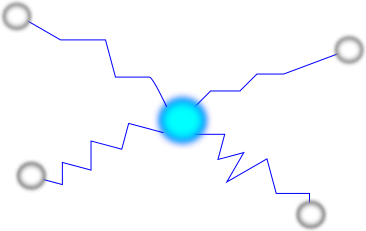
\includegraphics[width=150px, height=130px]{atomo.png}\label{osciladoratomico}\\

Figura \ref{osciladoratomico}. Modelo clásico de electrones ligados en un átomo. Los electrones son representados por círculos de fondo blanco, mientras que el circulo negro representa el núcleo. Los electrones están atados a el núcleo por resortes que representan las fuerzas de amortiguamiento entre ellos.
\end{center}

La frecuencia natural de resonancia $w_{0}$ de los dipolos atómicos esta determinado por su masa y la magnitud de la fuerza restauradora experimentada por pequeños desplazamientos. La masa apropiada es la masa reducida dada por:
\begin{equation}
\frac{1}{\mu}=\frac{1}{m_{0}}+\frac{1}{m_{N}}
\end{equation}
Donde $m_{0}$ y $m_{N}$ son las masas del electrón y del núcleo respectivamente, y ya que $m_{N}>>m_{0}$ se puede tomar $\mu\approx m_{0}$. La fuerza de amortiguamiento esta cuantificada en términos de la constante $K_{s}$,la cual esta dada cuando $w_{0}$ coincida con la frecuencia natural de los átomos:
\begin{equation}\label{frecuencia natural}
w_{0}=\sqrt{\frac{K_{s}}{\mu}}
\end{equation}
Tenemos que suponer que existen varios dipolos dentro de cada átomo para tomar en cuenta el hecho de que en un átomo dado pueden haber muchas frecuencias de transición. Estas se conocen de los espectros de emisión y transmisión, y las frecuencias ocurren en regiones del espectro infrarrojo cercano, visible y ultravioleta.

Podemos entender los dipolos atómicos  considerando las oscilaciones del dipolo mostrado en la figura \ref{oscilador}. Un dipolo eléctrico consiste en una carga positiva $+q$ en la posición $r_{+}$ y una carga negativa $-q$ en $r_{-}$. El momento dipolar eléctrico esta definido como:
\begin{equation}
p=q(r_{+}-r_{-})
\end{equation}

\begin{center}
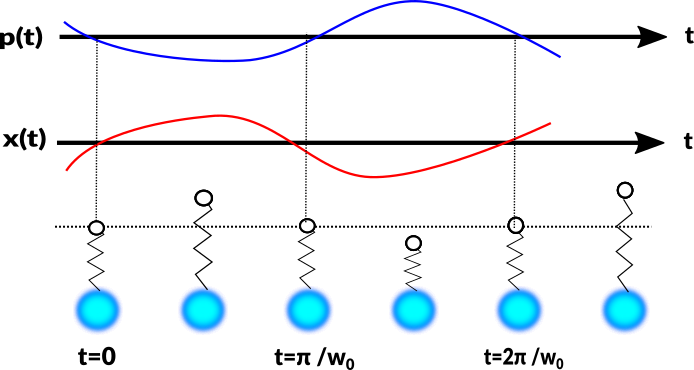
\includegraphics[width=330px, height=250px]{oscilador.png}\label{oscilador}\\

Figura \ref{oscilador}. Oscilaciones de un dipolo clásico consiste de una carga positiva pesada y una carga ligera negativa atados por un resorte. x(t) es la dependencia del desplazamiento de la carga negativa desde su posición de equilibrio. Las vibraciones naturales del dipolo sobre su posición de equilibrio a frecuencia $w_{0}$ genera un momento dipolar dependiente del tiempo p(t). \cite{MarkFox}.
\end{center}


Por lo tanto el núcleo positivo y el electrón negativo forman un dipolo con magnitud igual a $e|r_{N}-r_{e}|$.

Durante las oscilaciones del dipolo atómico, el núcleo se mantiene mas o menos estacionario debido a masa pesada, mientras que el electrón oscilara a frecuencia $w_{0}$. Por lo tanto las oscilaciones producen un dipolo variante en el tiempo en adicional a cualquier dipolo permanente que el átomo pueda tener. La magnitud del dipolo variante en el tiempo esta dado por:
\begin{equation}\label{momentoDipolar}
p(t)=-ex(t)
\end{equation}

Donde x(t) es el desplazamiento variante del electrón de su posición de equilibrio. Esta conexión entre el desplazamiento del electrón y la dependencia del dipolo atómico es mostrada en la figura[x]. El dipolo oscilante radia ondas electromagnéticas a frecuencia $w_{0}$, de acuerdo con la teoría de dipolos clásicos de Hertz. Por lo tanto el átomo se espera que radia luz a su frecuencia de resonancia cual sea que sea la energía impartida para excitar las oscilaciones.

También podemos usar el modelado dipolar para entender como los átomos interactúan con una onda electromagnética  de frecuencia w. El campo eléctrico ejerce fuerzas en el electrón y en el núcleo e induce al sistema a una frecuencia w. Si w coincide con una frecuencia natural del átomo, entonces tenemos un fenómeno de resonancia. Esto induce amplitudes altas en las oscilaciones. Los átomos sin embargo puede absorber energía de la onda de luz si $w=w_{0}$. La fuerza de absorción esta caracterizada por el coeficiente de absorción $\alpha$, y la intensidad de la onda decaerá exponencialmente de acuerdo a la ley de Beer.

Conocemos de la teoría cuántica lo que realmente sucede durante la absorción, el átomo saltara a un estado exitado por absorber un fotón. Esto puede ocurrir solo si $\hbar w=E_{2}-E_{1}$ donde $E_{1}$ y $E_{2}$ son las energías cuantizadas de los estados iniciales y final. Una ves que ha sido excitado, el átomo puede regresar a su estado base por una serie de transiciones de radiación, en el cual la energía de fotón absorbido es convertido en calor. Alternativamente puede haber luminiscencia remitiendo un fotón tiempo después. Los fotones re-irradiados son incoherentes entre ellos y son emitidos en todas las direcciones mas que en la dirección especifica del la onda incidente.  Por lo que hay un reducción en el flujo de energía en la direccioné del rayo, que es equivalente a la absorción.

Si w no coincide con ninguna frecuencia de resonancia, entonces los átomos no absorberán, y el medio sera transparente. En esta situación la luz  impulsara oscilaciones no resonantes a los átomos a su propia frecuencia w. Las oscilaciones de los átomos serán impulsados por la onda, pero con una fase de retraso. La fase de retraso es una característica de oscilaciones forzadas y es causada por el amortiguamiento. Los átomos oscilantes todos irradian instantáneamente, pero el retraso que se adquiere se acumula en el proceso y retarda la propagación del frente de onda. Esto implica que la velocidad de propagación es menor que en el espacio libre. Esta reducción de la velocidad en el medio es caracterizado por el índice de refracción.

La reducción de la velocidad de la onda debido a interacción no resonante puede ser considerada como un proceso de repetido de dispersión. La dispersion es ambas coherente y elástica, y cada átomo se comporta como una fuente de punto Huygens. La dispersión de la luz interfiere constructiva mente en la dirección de propagación y destructivamente en las demás, así que la dirección de propagación no cambia por dispersiones repetidas. Sin embargo cada evento de dispersión introduce un retraso en el tiempo lo cual causa que la propagación del frente de onda a través del medio sea mas lento.

\subsection{Osciladores Vibracionales}
Un medio óptico puede contener otros tipos de osciladores dipolares en adición a aquellos electrones ligados a los átomos. Si el medio es ionico, contendrá iones opuestos cargados. Las vibraciones de estos átomos cargados a partir de sus posiciones de equilibrio dentro de la red cristalina producirán momentos dipolares oscilantes, de la misma manera que lo hacen los átomos considerados anteriormente. Sin embargo, debemos también considerar los efectos ópticos debidos a estos osciladores vibracionales cuando consideramos la interacción de la luz con un medio óptico ionico.

Los efectos ópticos de osciladores vibracionales es bien conocido en física molecular. La figura\ref{modeloclasico} da una ilustración esquemática de una molécula polar clásica. Esta consiste de dos átomos cargados ligados entre ellos en una configuración estable, el resorte representa los enlaces moleculares entre ellos. Los átomos cargados pueden vibrar sobre su posición de equilibro e inducir  oscilaciones de manera análoga a los electrones ligados en los átomos. 


\begin{center}
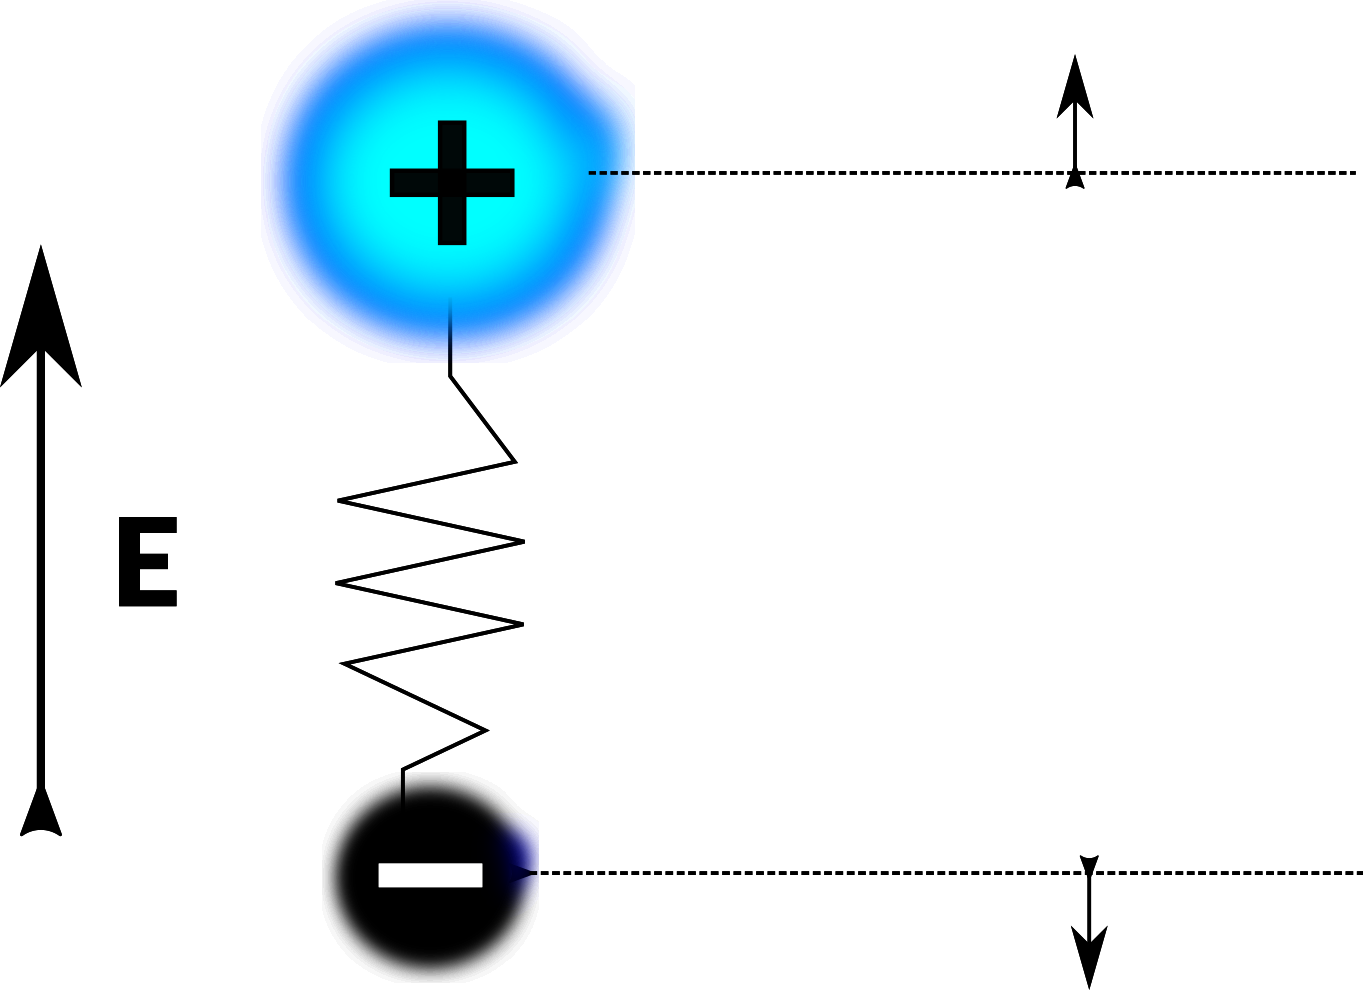
\includegraphics[width=150px, height=150px]{modeloclasico.png}\label{modeloclasico}\\

Figura \ref{modeloclasico}. Modelo clásico de una molécula polar. Los átomos están cargados positiva y negativamente, y pueden vibrar sobre sus posiciones de equilibrio. Estas vibraciones producen un campo eléctrico oscilantes que radiara ondas electromagnéticas a frecuencias de resonancia. Alternativamente, la molécula interactuara con el campo eléctrico E de la onda de luz a través de fuerzas ejercidas en los átomos cargados \cite{MarkFox}.
\end{center}

De la ecuación \ref{frecuencia natural} se puede ver que las vibraciones ocurrían a bajas frecuencias porque la masa reducida es mas grande. Las vibraciones sin embargo ocurren a frecuencias infrarrojas con $w/2\pi\approx 10^{12}-10^{13}$. Estamos vibraciones moleculares están asociadas con fuertes lineas de absorción en la región del espectro infrarrojo.

La interacción entre las vibraciones de la molécula y la onda de luz ocurre a través de fuerzas ejercidas en los átomos por el campo eléctrico. Es obvio que esto solo puede pasar si los átomos están cargados. 
En un solido cristalino formado de la condensación de moléculas polares, los átomos son arreglados en secuencia alternante de iones positivos y negativos. Los iones pueden vibrar sobre sus posiciones de equilibro, y esto produce oscilaciones dipolares. Estas oscilaciones están asociadas con vibraciones de la red, y pueden ocurrir a frecuencias en el espectro infrarrojo. 

La interacción de luz y materia esta asociada con las excitaciones de fonones, lo cuales cuantifican las vibraciones de red. A este estado podemos simplemente notar que las vibraciones de red de un cristal polar lleva a fuertes efectos ópticos en el rango del espectro infrarrojo. Estos efectos ocurrirán en adición a los electrones ligados a los átomos que componen el cristal. En la practica podemos tratar estos dos tipos de dipolos separadamente porque las resonancias son agudas y ocurren a diferentes frecuencias. Sin embargo los efectos resonantes de los electrones son despreciados a frecuencias de vibraciones de red y vice versa. 

\subsection{Electrones libres}
Los dipolos electrónicos y vibracionales considerados anteriormente son ejemplos de osciladores ligados. Los metales y semiconductores dopados en contraste contienen un significante numero de electrones libres. Como el nombre implica, estos son electrones que no están ligados a ningún átomo, y por lo tanto no experimentan fuerzas restauradoras cuando se desplazan. Estos implica que la constante de amortiguamiento en la ecuación \ref{frecuencia natural} es cero, y por lo tanto la frecuencia de resonancia es $w_{0}=0$.

El modelo de electrones libres en metales es atribuido a Paul Drude, y así la aplicación de el modelo de oscilador dipolar  a electrones libre es llamado modelado Drude Lorentz. El modelado de oscilador dipolar es perfectamente valido pero debemos poner $w_{0}=0$.

\section{El modelo oscilador dipolar}
En las secciones anteriores introducimos características generales del oscilador dipolar. Ahora queremos usar el modelo para calcular la dependencia de la frecuencia del índice de refracción y el coeficiente de absorción. Esto dará una explicación simple para la dispersión del índice de refracción en materiales ópticos, y también ilustrara un punto general de que el fenómeno de absorción y refracción están relacionados entre si.
\subsection{El oscilador Lorentz}
Hemos considerado la interacción de una onda electromagnética y un átomo con una simple frecuencia de resonancia $w_{0}$ debido a los electrones ligados, dado por la ecuación \ref{frecuencia natural}. El desplazamiento de dipolos atómicos son modelados como osciladores armónicos amortiguados. La inclusión del amortiguamiento es consecuencia del hecho de que los dipolos oscilantes pueden perder su energía en procesos de colisión. En solidos típicamente ocurre a través de la interacción con un fotón el cual ha sido termalmente excitado en el cristal. Como vimos anteriormente el termino de amortiguamiento tiene el efecto de reducir el pico del coeficiente de absorción y el ampliamiento de las lineas de absorción.

El campo eléctrico de la onda de luz induce oscilaciones forzadas al dipolo atómico a través de fuerzas de conducción ejercidas en los electrones. Se pondrá la condición de que $m_{N}>>m_{0}$ así podemos ignorar el movimiento del núcleo. El desplazamiento x del electrón esta gobernado por una ecuación de movimiento de la forma:
\begin{equation}\label{EcuacionOscilador}
m_{0}\frac{d^{2}x}{dt^{2}}+m_{0}\gamma\frac{dx}{dt}+m_{0}w_{0}^{2}x=-eE
\end{equation}
Donde $\gamma$ es el índice de amortiguamiento, $e$ es la magnitud de la carga eléctrica del electrón, y E es campo eléctrico de la onda de luz. El termino del lado izquierdo representa la aceleración, el amortiguamiento y la fuerza restauradora respectivamente. El amortiguamiento es modelado por una fuerza de fricción la cual es proporcional a la velocidad y la reducción del movimiento. El termino del lado derecho representa la fuerza de conducción debido a el campo eléctrico alternante de la onda de luz.
Consideraremos la interacción del átomo con una onda de luz monocromática de frecuencia angular w. La dependencia en el tiempo del campo eléctrico esta dado por:
\begin{equation}\label{campoE}
E(t)=E_{0}cos(wt+\phi)=E_{0}Re(exp(-iwt-\phi))
\end{equation}
Donde $E_{0}$ es la amplitud y $\phi$ es la fase de la luz. Con el fin de mantener consistencia con la convención de signos, se ha escogido tomar la parte de la frecuencia negativa de la exponencial compleja.
El campo eléctrico alternante inducirá movimientos oscilantes a frecuencia w. Sin embargo sustituyendo la ecuación \ref{campoE} en la ecuación \ref{EcuacionOscilador}, encontramos que la solución es de la forma:
\begin{equation}\label{SolucionOscilador}
x(t)=X_{0}Re(exp(-iwt-\phi^{'}))
\end{equation}
Donde $X_{0}$ y $\phi^{'}$ son la amplitud y fase de las oscilaciones. Podemos incorporar los factores de fase de las ecuaciones \ref{campoE} y \ref{SolucionOscilador} en las amplitudes permitiendo que $E_{0}$ y $X_{0}$ sean números complejos. Entonces sustituimos $E(t)=E_{0}e^{-iwt}$ en \ref{EcuacionOscilador} encontrando que la solución es de la forma $x(t)=X_{0}e^{-iwt}$. Esto da:
\begin{equation}
-m_{0}w^{2}X_{0}e^{-iwt}-im_{0}\gamma wX_{0}e^{-iwt}+m_{0}w_{0}^{2}X_{0}e^{-iwt}=-eE_{0}e^{-iwt}
\end{equation}
Lo cual implique que:
\begin{equation}
X_{0}=\frac{-e E_{0}/m_{0}}{w_{0}^{2}-w^{2}-i\gamma w}
\end{equation}
El desplazamiento de los electrones desde su posición de equilibrio produce un momento dipolar variante $p(t)$. La magnitud del dipolo esta dado por la ecuación \ref{momentoDipolar}. Esto da una contribución resonante a la polarización macroscópica(momento dipolar por unidad de volumen) en el medio.

Si N es el numero de átomos por unidad de volumen, la polarización resonante da:
\begin{equation}\label{Presonante}
P_{resonante}=Np=-Nex=\frac{Ne^{2}}{m_{0}}\frac{1}{w_{0}^{2}-w^{2}-i\gamma w}E
\end{equation}
Una rápida inspección de esta ecuación muestra que la magnitud de $P_{resonante}$ es pequeña a menos que la frecuencia sea cercana a $w_{0}$. Esto es otra propiedad general de oscilaciones forzadas, la respuesta es pequeña amenos que la frecuencia sea cercana a la frecuencia natural del oscilador.

La ecuación \ref{Presonante} puede ser usada para obtener la función dieléctrica $\varepsilon$. El desplazamiento eléctrico D del medio esta relacionado con el campo eléctrico E y la polarización P a través:
\begin{equation}\label{ecuacion211}
D=\varepsilon_{0}E+P
\end{equation}
Donde D, E y P son vectores. Estamos interesados en la respuesta optica a frecuencias cercanas a $w_{0}$ y asi dividimos la polarizacion en una parte resonante y un termino no resonante. Entonces podemos escribir:
\begin{equation}\label{ecuacion212}
D=\varepsilon_{0}E+P_{no-resonante}+P_{resonante}=\varepsilon_{0}E+\varepsilon_{0}\chi E+P_{resonante}
\end{equation}
Para simplificar la matemática, asumiremos que el material es isotropico, en el cual la función dieléctrica es definida a través de la relación:
\begin{equation}\label{relacionC}
D=\varepsilon_{0}\varepsilon E
\end{equation}
Entonces combinando las ecuaciones \ref{Presonante} y \ref{relacionC} se obtiene:
\begin{equation}
\varepsilon(w)=1+\chi +\frac{N e^{2}}{\varepsilon_{0}m_{0}}\frac{1}{(w_{0}^{2}-w^{2}-i\gamma w)}
\end{equation}
Esta puede ser dividida en sus partes reales e imaginarias:
\begin{equation}\label{var1lorentz}
\varepsilon_{1}(w)=1+\chi+\frac{Ne^{2}}{\varepsilon_{0}m_{0}}\frac{w_{0}^{2}-w^{2}}{(w_{0}^{2}-w^{2})^{2}+(\gamma w)^{2}}
\end{equation}
\begin{equation}\label{var2lorentz}
\varepsilon_{2}(w)=\frac{Ne^{2}}{\varepsilon_{0}m_{0}}\frac{\gamma w}{(w_{0}^{2}-w^{2})^{2}+(\gamma w)^{2}}
\end{equation}

Estas formulaciones pueden simplificarse aun mas si estamos trabajando con frecuencias cercanas a la frecuencia de resonancia, donde $w\approx w_{0}>>\gamma$. Esto permite aproximar $(w_{0}^{2}-w^{2})$
por $2w_{0}\nabla w$, donde $\nabla w=(w-w_{0})$ es la diferencia desde $w_{0}$. Podemos notar que los limites de bajas y altas frecuencias de $\varepsilon(w)$ esta dado por:
\begin{equation}
\varepsilon(0)=\varepsilon_{st}=1+\chi +\frac{Ne^{2}}{\varepsilon_{0}m_{0}w_{0}^{2}}
\end{equation} 
y a altas frecuencias:
\begin{equation}
\varepsilon(\infty)=\varepsilon_{\infty}=1+\chi
\end{equation}
Las etiquetas de $\varepsilon_{st}$ es por estático, ya que representa la respuesta del dieléctrico a campos eléctricos estáticos. Con esta notación encontramos que:
\begin{equation}\label{ecuacion219}
(\varepsilon_{st}-\varepsilon_{\infty})=\frac{Ne^{2}}{\varepsilon_{0}m_{0}w_{0}^{2}}
\end{equation}
Podemos reescribir las ecuaciones \ref{var1lorentz} y \ref{var2lorentz} en la siguiente forma valida a frecuencias cercanas a la resonancias:
\begin{equation}\label{var1Delta}
\varepsilon_{1}(\Delta w)=\varepsilon_{\infty}-(\varepsilon_{st}-\varepsilon_{\infty})\frac{2w_{0}\Delta w}{4(\Delta w)^{2}+\gamma^{2}}
\end{equation}
\begin{equation}\label{var2Delta}
\varepsilon_{2}(\Delta w)=(\varepsilon_{st}-\varepsilon_{\infty})\frac{\gamma w_{0}}{4(\Delta w)^{2}+\gamma^{2}}
\end{equation}

Estas ecuaciones describen una aguda linea de absorción centrada en $w_{0}$ con un ancho en la mitad de la caída igual a $\gamma $.

La figura \ref{graficas} muestra la dependencia de $\varepsilon_{1}$ y $\varepsilon_{2}$ predicha por las ecuaciones \ref{var1Delta} y \ref{var2Delta} para un oscilador con $w_{0}=10^{14}Hz$, $\gamma=5\times 10^{12}Hz$, $\varepsilon_{st}=12.1$ y $\varepsilon_{\infty}=10$. Estos números son bastantes típicos para lineas de absorción en el infrarrojo de un cristal ionico. Se ve que $\varepsilon_{2}$ es un fuerte pico de absorción que depende de la frecuencia $w$ con un valor máximo en $w_{0}$ y un ancho total igual a la mitad del valor máximo igual a $\gamma $. La dependencia de $\varepsilon_{1}$ es mas complicada, a medida que se acerca por debajo a $w_{0}$ gradualmente se eleva desde el valor de baja frecuencia $\varepsilon_{st}$ y alcanza un pico en $w_{0}-\gamma /2$ y entonces decae rápidamente formando un pico en $w_{0}+\gamma /2$ antes de alcanzar la frecuencia $\varepsilon_{\infty}$.

\begin{center}
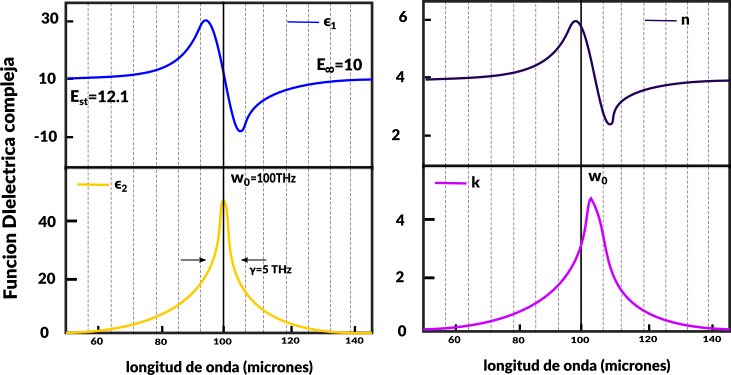
\includegraphics[width=380px, height=250px]{graficas.png}\label{graficas}\\

Figura \ref{graficas}. Dependencia de la frecuencia de las partes reales e imaginarias de la función dieléctrica compleja de un oscilado dipolar a frecuencias cercanas a la resonancia. Los gráficos están calculados para un oscilador con $w_{0}=100THz$,$\gamma =5 THz$, $\varepsilon_{st}=12.1$ y $\varepsilon_{\infty}=10$(1 $THz=10^{12}H$), también  se muestran el índice de refracción y el coeficiente de extinción calculador a partir de la función dieléctrica \cite{MarkFox}.
\end{center}

Notemos que la escala de frecuencia sobre la cual estos efectos están ocurriendo esta determinado por $\gamma$ para ambos $\varepsilon_{1}$ y $\varepsilon_{2}$. Esto muestra que el amortiguamiento de los osciladores causa el ensanchamiento de los picos. La dependencia de frecuencia determinada por $\varepsilon_{1}$ y $\varepsilon_{2}$ mostrada en la \ref{graficas} es llamada Lorentziano.

En un experimento usualmente se mide el índice de refracción $n$ y el coeficiente de absorción $\alpha$. La medición de $\alpha$ entonces permite determinar el coeficiente de extinción $k$. La figura \ref{graficas} muestra los valores de n y k calculados a partir de $\varepsilon_{1}$ y $\varepsilon_{2}$ usando las ecuaciones \ref{var1Delta} y \ref{var2Delta}. Vemos que $n$ sigue aproximadamente la dependencia de frecuencia de $\sqrt{\varepsilon_{1}(2)}$ mientras que $k$ mas o menos se comporta como $\varepsilon_{2}$. La correspondencia $n\alpha\sqrt{\varepsilon_{1}}$ y $k\alpha\varepsilon_{2}$ seria exacta si $k$ fuese mucho menor que $n$, que generalmente sucede en gases en los cuales la baja densidad de átomos hace que la absorción total sea pequeña.

Un aspecto interesante del oscilador Lorentz es que el índice de refracción se ve afectado sobre un rango de frecuencias mayor que la absorción.

\subsection{Múltiples Resonancias}
En general, un medio óptico tendrá muchas frecuencias características resonantes. Ya observamos que sucede para frecuencias naturales resonantes individuales esto debido a vibraciones de red y electrones ligados dentro de los átomos. Sin embargo un medio puede tener muchas frecuencias resonantes de cada tipo. Podemos tratas estas múltiples resonancias sin dificultad en nuestro modelo teniendo en cuenta que ocurren a distintas frecuencias.
Anteriormente dividimos la polarización del medio en una parte resonante y una no resonante. Entonces se discutió la parte resonante en detalle, sin especificar con mucha precisión que significaba el termino no resonante. Simplemente se estableció que $P$ era proporcional a $E$ a través de la susceptibilidad $\chi$. En realidad, la polarización no resonante del medio debe originarse desde la polarizabilidad de los átomos exactamente de la misma manera que la parte resonante. La ecuación \ref{ecuacion219} nos dice que la constate dieléctrica disminuye cada vez que se atraviesa una linea de absorción. Las contribuciones que entran en la susceptibilidad eléctrica de fondo $\chi$ en la ecuación \ref{ecuacion212} entonces surgen de la polarización debido a otros osciladores a altas frecuencias.
Podemos entender este punto mejor haciéndolo mas cuantitativo. La contribución de la polarización de un oscilador particular es dado por la ecuación \ref{Presonante}. En un medio con muchos osciladores electrónicos de diferentes frecuencias la polarización estaría dada por :
\begin{equation}
P=(\frac{Ne^{2}}{m_{0}}\sum_{j}\frac{1}{(w_{j}^{2}-w^{2}-i\gamma_{j}w)})E
\end{equation}
Donde $w_{j}$ y $\gamma_{j}$ son las frecuencias y los términos de amortiguamiento de una resonancia particular. Entonces sustituimos esto en la ecuación \ref{Presonante}  y utilizamos la definición de $\varepsilon$ dada en la ecuación \ref{relacionC}. Esto da:
\begin{equation}\label{ecuacion223}
\varepsilon(w)=1+\frac{Ne^{2}}{\varepsilon_{0}m_{0}}\sum_{j}\frac{1}{(w_{j}^{2}-w^{2}-i\gamma_{j}w)}
\end{equation}
Esta ecuación toma en cuanto todas las transiciones del medio y puede ser usada para calcular la dependencia completa de la constante dieléctrica.

\begin{center}
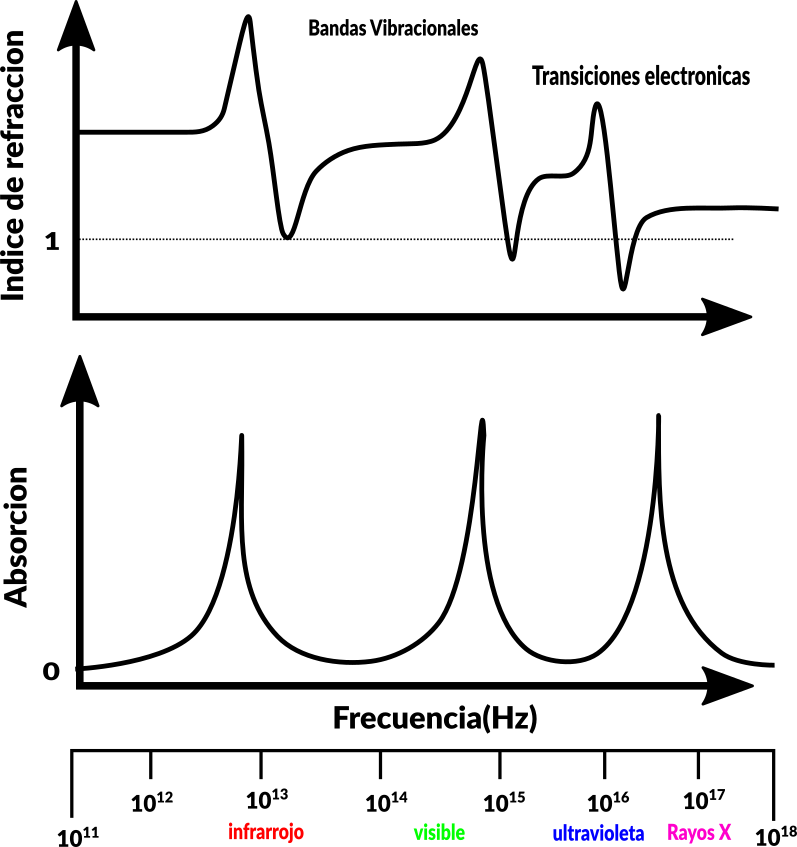
\includegraphics[width=380px, height=320px]{multi.png}\label{multi}\\

Figura \ref{multi}. Diagrama esquemático de la dependencia del índice de refracción y la absorción de un solido hipotético desde la región espectral infrarroja hasta los rayos X. El solido posee tres frecuencias de resonancia fundamentales $4\times 10^{13}Hz$,$4\times 10^{15}Hz$, $1\times 10^{17}Hz$ respectivamente. 
\end{center}

El índice de refracción y el coeficiente de absorción calculado de la ecuación \ref{ecuacion223} son graficados en función de la frecuencia en la figura \ref{multi}. La figura ha sido calculado para un solido hipotético con tres resonancias bien separadas con $w_{j}$ igual a $4\times 10^{13}Hz$,$4\times 10^{15}Hz$ y $1\times 10^{17}Hz$ respectivamente. El ancho de cada linea de absorción ha sido puesta al $10\%$ del centro de frecuencia por una apropiada elección del termino de amortiguamiento. La resonancia en el infrarrojo esta incluida para representar la absorción vibracional. En un solido real podemos adaptar el modelo para tomar en cuanto las diferentes masas reducidas y la carga efectiva de los osciladores vibracionales.

Podemos entender esta figura empezando desde altas frecuencias y gradualmente trabajándolo bajando a frecuencias mas bajas. En las frecuencias mas altas, los electrones son incapaces de responder al campo de conducción. El medio sin embargo no tiene polarización, y la constante dieléctrica es la unidad. A medida que se reduce la frecuencia, primero pasamos a las transiciones de los electrones internos en los rangos espectrales ultravioleta y rayos X, y así las transiciones de los electrones mas externos el ultravioleta y visible. Entonces tenemos una región donde no hay transiciones hasta que finalmente alcanzan las frecuencias vibracionales en el infrarrojo. Cada vez que pasamos a través de las resonancia se ve la característica dependencia de la frecuencia del oscilador Lorentz, con un pico en el espectro de absorción y una sacudida en el índice de refracción.

Dentro de estas resonancias el medio es transparente, el coeficiente de absorción es cero y el índice de refracción es casi constante.
El valor del índice de refracción en regiones transparentes gradualmente aumenta a medida que atraviesa linea de resonancia y la frecuencia disminuye. Este aumento del índice de refracción es causado por el hecho de que $\varepsilon_{st}>\varepsilon_{\infty}$ (ecuación \ref{ecuacion219}), lo cual implica que es $n$ es mayor por de bajo de una linea de absorción que sobre ella. 

Haciendo referencia a la figura \ref{multi} se puede ver que debemos entender el $'estatico'$ y el $'\infty ' $ relativo a una resonancia en particular. La variación de $n$ con la frecuencia debido a las resonancias es originado por la dispersión  encontrada en materiales ópticos incluso cuando son transparentes. 

EL oscilador dipolar predice que cada oscilador contribuye un termino dado por la ecuación \ref{Presonante}, esto lleva a una seria de lineas de absorción de la misma fuerza. Sin embargo datos experimentales muestran que la fuerza de la linea de absorción varia considerablemente entre distintas transiciones atómicas. Esto es causado por la variación de las probabilidades de transiciones mecánico cuánticas. En física clásica, sin embargo no hay explicación. y podemos asignar una fuerza del oscilador fenomenológica  $f_{j}$ a cada transición, reescribiendo la ecuación \ref{ecuacion223} como:
\begin{equation}
\varepsilon(w)=1+\frac{Ne^{2}}{\varepsilon_{0}m_{0}}\sum_{j}\frac{f_{j}}{(w_{0j}^{2}-w^{2}-i\gamma_{j} w)}
\end{equation}
Se puede demostrar por mecánica cuántica que debemos tener $\sum_{j} f_{j}=1$ para cada electrón. Y ya que el modelado clásico predice  que $f_{j}=1$ para cada oscilador,  podemos interpretar esto diciendo que cada electrón particular esta envuelto en varias transiciones al mismo tiempo, y la fuerza de absorción esta siendo dividida entre estas transiciones.
\subsection{Comparación con datos experimentales}
El comportamiento esquemático mostrado en la figura \ref{multi} puede ser comparado con datos experimentales típicos de un material en estado solido. La figura \ref{experimento} muestra la dependencia de la frecuencia del índice de refracción y el coeficiente de extinción del vidrio (silicio fundido $SiO_{2}$) desde el rango del infrarrojo hasta la región espectral de los rayos X.

Las características generales indicadas de la figura \ref{multi} puede ser observadas claramente, con fuerte absorción en el infrarrojo y ultravioleta y una amplia región de baja absorción entre ellos. Los datos confirman que $n>>k$ excepto cerca de los picos de absorción. Esto significa que las aproximaciones son totalmente validas en este rango.

La figura \ref{experimento} es típica de materiales los cuales son transparentes en la región del espectro visible. Anteriormente se menciono que el rango de transmisión de materiales descoloridos esta determinado por la absorción electrónica en el ultravioleta y las absorciones vibracionales en el infrarrojo. 
\begin{center}
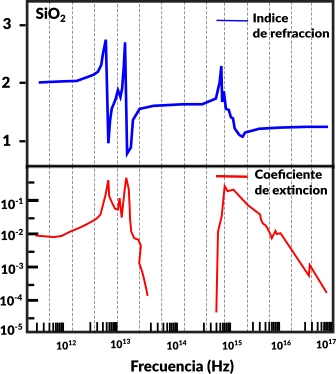
\includegraphics[width=380px, height=400px]{experimento.png}\label{experimento}\\

Figura \ref{experimento}. a) Índice de refracción b) coeficiente de extinción del silicio fundido ($SiO_{2}$) desde la región infrarrojo hasta los rayos X.\cite{MarkFox}
\end{center}

El silicio es un vidrio, y por lo tanto no tiene ninguna red cristalina regular. La absorción infrarrojo es sin embargo causada por excitación de cuantos vibraciones en las moléculas del $SiO_{2}$. Dos picos bien definidos se observan en $1.4\times 10^{13}Hz$ $21\mu m$ y $3.3\times 10^{13}Hz$ (9.1 $\mu m$) respectivamente. Estos corresponden a diferentes modos vibraciones de la molécula. 

La absorción ultravioleta en el silicio es causada por transiciones electrónicas interbandas. El silicio tiene un banda de energía sobre los $10ev$, y las transiciones interbandas son posibles cual sea la energía del photon que exceda este valor. Por lo tanto se observa un umbral en el ultravioleta en $2\times 10^{15}Hz$ (150nm).

Los picos de absorción interbandas al rededor de $ 3 \times  10^{16}Hz$ y $1.3 \times 10^{17} Hz$, son causados por las transiciones de los electrones del núcleo interno de los átomos del silicio y del oxígeno. El hecho de que la absorción electrónica consiste de un continuo de bandas mas que lineas discretas es difícil de modelar con precision por oscilador Lorentz. 
Los datos en la figura\cite{experimento} muestran que el índice de refracción decae por debajo de la unidad a un numero de frecuencias. Esto implica que la velocidad de fase de la luz es mayor que c, lo cual parece implicar una contradicción con la relatividad. Sin embargo, se sobrepone el hecho de que la señal debe ser transmitida como un paquete de ondas mas que una onda monocromática. En un medio dispersivo, un paquete de onda se propagara a la velocidad de grupo $v_{g}$ dada por:

\begin{equation}
v_{g}=\frac{dw}{dk}
\end{equation}

Y la velocidad de fase $v=w/k=c/n$. La relación entre la velocidad de grupo $v_{g}$ y la velocidad de fase $v$ es:
\begin{equation}
v_{g}=v(1-\frac{k}{n}\frac{dn}{dk})
\end{equation}
El termino $dn/dk$ es positivo en la mayoría de materiales bajo frecuencias ópticas. Esto entonces implica que la velocidad de grupo $v_{g}$ es siempre menor que $v$ y si intentamos transmitir una señal en la región del espectro donde $v>c$, podemos encontrar que $v_{g}$ es menor que c. 


\section{Análisis variacional Kramers Kronig restringido}

\subsection{Modelado básico de datos ópticos}
El análisis de datos experimentales es un proceso en el cual se utiliza una función matemática modelo que represente un fenómeno físico. Esta función modelo contara con un conjunto de parámetros ajustables, los cuales pueden variar con el fin de encontrar la mejor aproximación a los datos experimentales. Encontrar un modelo apropiado usualmente es el problema central, que la computadora difícilmente puede lograr. Una vez que tenemos el modelo con los valores iniciales seleccionados lo siguiente es ajustarlos.

Supongamos que tenemos un conjunto N de puntos experimentales \{$x_{i}, y{i}, \sigma_{i}$\} $(i=1...N)$ que queremos acoplar. Aquí $x_{i}$ es el dato coordenada, $y_{i}$ es el dato valor y $\sigma_{i}$ es la barra de error. Ahora tomamos un modelo que calcule $y$ en función de $x$,  y unos parámetros internos \{$p_{1},p_{2}..p_{m}$\} $y=f(x,p_{1}..p_{m})$.\

Entonces construimos el funcional ``chi-cuadrado":\\

\begin{equation}
 \chi^{2}=\sum_{i=1}^{N}(\frac{y_{i}-f(x_{i},p_{1}..p_{M})}{\sigma_{i}})^{2} 
\end{equation}

Si asumimos que todos los valores medidos $y_{i}$ están normalmente distribuidos con desviación estándar dada por $\sigma_{i}$, entonces estadísticamente  el mejor ajuste sera en el valor mínimo de $\chi^{2}$. Así el modelado es esencialmente la minimización de ``chi-cuadrado", sin embargo el método en si mismo es llamado mínimos cuadrados\cite{guide}.\\
En cuanto $f(x,p_{1}..p_{m})$ es una función no lineal de parámetros, usaremos el llamado algoritmo Levenberg-Marquardt para la minimización de ``chi-cuadrado".

\subsection{Algoritmo Levenberg-Marquardt}
Este algoritmo es usado para resolver problemas de mínimos cuadrados no lineales, se basa en el balance auto-ajustable entre dos técnicas de minimización, el gradiente descendente y el inverso hessiano. El método del gradiente descendente es simplemente el movimiento de la curva en la dirección de descenso mas aguda la cual esta determinada por el gradiente:\\
\begin{equation}
\beta_{k}=\frac{-1}{2}\frac{\partial\chi^{2}}{\partial p_{k}}=\sum_{i=1}^{N}\frac{y_{i}-f(x,p_{1},..,p_{m})}{\sigma_{i}^{2}}\frac{\partial f}{\delta p_{k}}(x,p_{1},..,p_{M})
\end{equation}
Supondremos que los parámetros actuales son $p_{k}$ $(k=1..M)$.  Esta técnica se justifica cuando nos encontramos fuera de los mínimos de la curva ya que cerca de ellos la técnica es ineficiente. 
Para el caso de los mínimos  es mejor minimizar una función con forma parabólica, determinada por el Hessiano:
\begin{equation}
\alpha_{kl}=
\frac{1}{2}\frac{\partial^{2}\chi^{2}}{\partial p_{k}\partial p_{l}
}
\end{equation}
\begin{large}
\begin{center}
$
=\sum_{i=1}^{N}\frac{1}{\sigma_{i}^{2}}\{\frac{\partial f}{p_{k}}(x_{i},p_1..p_{M})\frac{\partial f}{\partial p_{1}}(x_{i},p_{1}..p_{M})-[y_{i}-f(x_{i},p_{1}..p_{M})]\frac{\partial^{2}f}{\partial p_{k}\partial p_{l}(x_{i},p_{1}..p_{M})}\}
$
\end{center}
\end{large}

Después de calcular el gradiente descendente y el Hessiano  para el conjunto actual de parámetros, inmediatamente saltamos al mínimo cambiando los parámetros $p_{k}->p_{k}+\delta p_{k}$, donde el vector desplazamiento $\delta p_{k}$ esta determinado por el sistema lineal.
\begin{equation}
\sum_{i=1}^{M}\alpha_{kl}\delta p_{l}=\beta_{k}
\end{equation}
El termino que contiene la segunda derivada de la función no es importante cerca del mínimo sin embargo puede desestabilizar el proceso de acoplamiento, así en vez de la ecuación 17 definimos la matriz:
\begin{equation}
\alpha_{kl}=\sum_{i=1}^{N}\frac{1}{\sigma_{i}^{2}}\frac{\partial f}{\partial p_{k}}(x_{i},p_{1}..p_{m})\frac{\partial f}{\partial p_{l}}(x_{i},p_{1}..p_{m})
\end{equation}
Devolviendo a la técnica del gradiente descendente, tenemos un problema con las unidades para ello normalizamos por $\alpha_{kk}$
\begin{equation}
\delta p_{k}=\frac{constante}{\alpha_{kk}}\times \beta_{k}
\end{equation}
Existe una manera para cambiar continuamente de una técnica a otra. 
\\
Consideremos la matriz mejorada:
\begin{equation}
\alpha'_{kl}=\alpha_{kl}(1+\delta_{kl}\lambda)
\end{equation} 
Donde $\lambda$ es una constante sin dimension, y remplazamos $\alpha_{kl}$ con $\alpha'_{kl}$ en la ecuación 18.
\begin{equation}
\sum_{i=1}^{M}\alpha'_{kl}\delta p_{l}=\beta_{k}
\end{equation}
Si tomamos $\lambda$<<1 el vector desplazamiento $\delta p_{k}$, obtenido por la ecuación 21 sera cercano a uno, obtenido puramente por la técnica del inverso Hessiano. Sin embargo si tomamos $\lambda$>>1 entonces podemos ignorar los elementos fuera de la diagonal y la solución de la ecuación 22 sera simplemente
\begin{equation}
\delta p_{k}=\frac{\beta_{k}}{\alpha'_{kk}}=\frac{\beta_{k}}{\alpha_{kk}(1+\lambda)}
\end{equation}
Por la forma de la ecuación  significa que aumentando el parámetro $\lambda$ nos acercamos al limite del ``descenso mas agudo".\\
\begin{center}

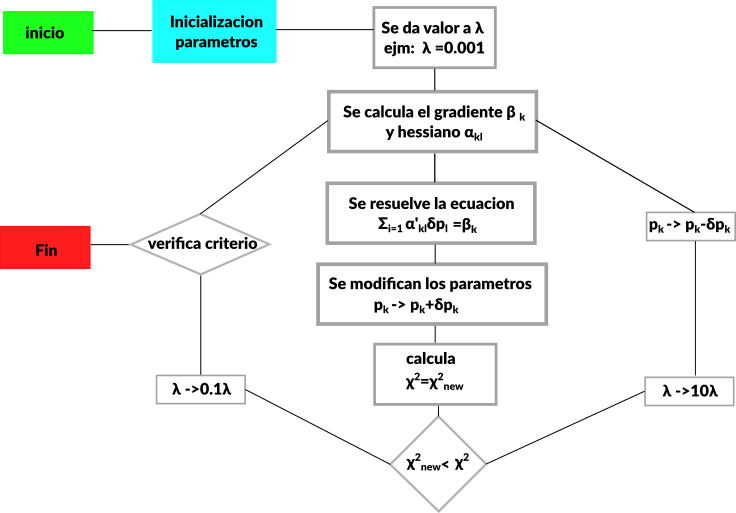
\includegraphics[width=400px, height=250px]{diagrama.png} \newline
Figura 4. Diagrama de algoritmo Levenberg-Marquardt.\\
\end{center}

La minimización es un proceso iterativo. Empezamos con un valor razonable de $\lambda$. A cada iteración exitosa ($\chi_{new}^{2}<\chi_{actual}^{2}$) se reduce en un factor de 10, moviéndose hacia el régimen del inverso Hessiano. De lo contrario ira hacia el régimen del  ``descenso mas agudo", aumentando landa en un factor de 10. Cuando se cumpla con el criterio de ajuste habrá terminado .
Un asunto importante es calculo de $\alpha_{kl}$ y $\beta_{k}$. De acuerdo a la ecuación 15 y 19, primero debemos calcular la primera derivada de la función modelo $f(x,p_{1},..,p_{M})$ con respecto a los parámetros. Usaremos modelos de funciones dadas por expresiones analíticas, podemos siempre calcular las derivadas analíticamente.
El criterio es necesario para detener la iteración del ciclo. La razón mas natural seria cuando el proceso de acoplamiento converja o formalmente cuando la reducción absoluta de $\chi_{2}$ durante las ultimas iteraciones no exceda cierto limite de confianza $\delta\chi^{2}$. También debemos asegurar que el proceso de acoplamiento no tome demasiado tiempo para ello ponemos algunos limites en el numero total de iteraciones o en el tiempo total del ajuste. A pesar de la simplicidad del algoritmo Levenberg-Marquardt es notable que puede fácilmente manejar modelos que contienen un gran numero de parámetros. La velocidad de convergencia o el numero de iteraciones necesarias para al alcanzar el mínimo no son significativamente por el numero de parámetros, esto depende mas bien de lo adecuado del modelo a los datos experimentales y de  la aproximación inicial\cite{guide}.

\subsection{Límites de confianza}
Cuando el acoplamiento esta completo, a menudo es necesario estimar las barras de error de los parámetros $p_{k}$ obtenidos, desde el punto de vista estadístico es mejor hablar de los llamados limites de confianza. Uno puede intuir el limite de confianza de un parámetro $p_{k}$ como pumo el valor mas grande posible de $\delta p_{k}$, tal que cuando el valor $pk\rightarrow p_{k}^{(0)}+\delta p_{k}$ cambie no cause un incremento irreal del termino chi-cuadrado. Es esencial agregar a esta definición que después de cambiar el valor de $p_{k}$, se debe minimizar $\chi^{2}$ con respecto a los parámetros restantes. La importancia de una minimizaciòn extra es clara desde el siguiente ejemplo\cite{guide}.

Consideremos la función modelo  $f$, la cual depende de dos parámetro($p_{1}$ y $p_{2}$), incluso vemos que no depende de $x$ esto es $f(p_{1},p_{2})=p_{1}+p_{2}$ suponga que nuestro conjuntos de puntos contiene \{$y=1,\sigma=1$\}, el termino chi-cuadrado sera $\chi^{2}=(1-p_{1}-p_{2})^{2}$. El procedimiento de ajuste puede converger por ejemplo a $p_{1}^{(0)}=0.6$ y $p_{1}^{(0)}=0.4$ (en este caso el ajuste es exacto $\chi^{2}=0$).
Obviamente estos parámetros no tienen limites ya que para cualquier numero a, la combinación $p_{1}=a,p_{2}=1-a.$ también provee un acoplamiento exacto. Sin embargo a un valor fijo de $p_{2}$ el cambio de $p_{1}$  causara un incremento de chi-cuadrado, Si nosotros ahora colocamos un valor realista a $\chi^{2}$ como 0.01 entonces formalmente el limite de confianza de $p_{1}$ debe ser 0.1. lo mismo es valido para $p_{2}$, se puede decir que los parámetros $p_{1}$ y $p_{2}$ están correlacionados.
El calculo de los limites de confianza $\delta p_{k}$ es relativamente sencillo. Podemos ignorar las desviaciones de $\chi^{2}(p_{1},..,p_{M})$ cerca del punto mínimo  $\chi_{(0)}^{2}(p_{1}^{(0)},..,p_{M}^{(0)})$ de la forma cuadrática, dado por la matriz Hessiana $\alpha_{kl}$\cite{guide}.

\begin{equation}
\chi^{2}-\chi_{(0)}^{2}=\sum_{k,l}\alpha_{kl}(p_{k}-p_{k}^{(0)})(p_{l}-p_{l}^{0})
\end{equation}
Sea $\delta\chi^{2}$ la diferencia $\chi^{2}-\chi_{(0)}^{2} $ máxima aceptable. Entonces se obtiene:
\begin{equation}
\delta p_{k}=\sqrt{(\delta \chi^{2})(\alpha^{-1})^{kk}}
\end{equation}
donde $ (\alpha^{-1})^{kl}$es la inversa de la matriz Hessiana también llamada "matriz de covariancia". Note que todos los elementos de la diagonal $ (\alpha^{-1})^{kk}$ son positivos porque $\chi_{(0)}^{2}=(p_{1}^{0},..,p_{m}^{0})$ es un punto mínimo local y la ecuación (25) puede ser siempre aplicada. Afortunadamente de la ecuación (25) se sigue que $\delta\chi^{2}$ escala los limites de confianza de todos los parámetros proporcionalmente. Por consiguiente se puede comparar de forma fiable las barras de error de diferentes parámetros a pesar de que sus valores puedan estar mal definidos\cite{guide}.
\chapter{Metodologia}

Para entender la definición formal del problema supongamos que queremos modelar un conjunto de medidas ópticas experimentales obtenidos por la técnica de reflectancia a incidencia normal $\{w_{i}, R_{i},\delta R{i} \} $ con $i= 1,..,N_{exp}$. Aquí $w_{i}$ es la frecuencia experimental, $R_{i}$ es valor experimental de la reflectancia  y  $\delta R_{i}$ es el error experimental.

El siguiente paso sera construir un conjunto de puntos frecuencias distinta al rango de frecuencias experimentales, la llamaremos malla de frecuencia $\{w_{k}^{malla}\}$ para $k=1,..,N_{exp}-2$ . Donde cada punto de la malla estará entre los puntos de frecuencia experimentales $w_{i}$ dados por: 
\begin{center}
$w_{k}^{malla}=\frac{w_{k+1}-w_{k}}{2}$  $para$ k $desde$ 1 $hasta$ $N-2.$
\end{center}
Asumiremos que todas las cantidades opticas pueden ser expresadas por una parte real y una imaginaria de la función de respuesta compleja. Ahora especifiquemos como sera el funcional modelo para $R(w)$.  Un buen candidato es una función modelo de forma triangular (Figura \ref{FuncionTriangular}) \cite{constrained}:


\begin{equation}
R_{k}^{\bigtriangleup}(w_{k}^{malla})=\left \{ \begin{array}{lcc}
\frac{w_{k}^{malla}-w_{k-1}}{w_{k}-w_{k-1}}&, si &w_{k-1}<w_{k}^{malla}<w_{k}\\
\\ \frac{w_{k+1}-w_{k}^{malla}}{w_{k+1}-w_{k}}&, si &w_{k}<w^{malla}_{k}<w_{k+1}\\
\\   0 &,  otros&casos\\
\end{array}
\right.
\end{equation}

El termino imaginario que corresponde al cambio de fase $\phi_{k}(w_{k}^{malla})$ puede ser obtenido analíticamente aplicando las transformaciones Kramers Kronig \cite{constrained}.

\begin{equation}
\phi_{k}^{\bigtriangleup}(w_{k}^{malla})=\frac{1}{\pi}[\frac{g(w_{k}^{malla},w_{k-1})}{w_{k}-w_{k-1}}-\frac{(w_{k+1}-w_{k-1})g(w^{malla}_{k},w_{k})}{(w_{k}-w_{k-1})(w_{k+1}-w_{k})}+\frac{g(w_{k}^{malla},w_{k+1})}{w_{k+1}-w_{k}}]
\end{equation}

Donde \\

\begin{equation}
g(x,y)=(x+y)ln\left |x+y\right | +(x+y)ln\left |x+y\right |
\end{equation}


\begin{figure}[H]
\begin{center}
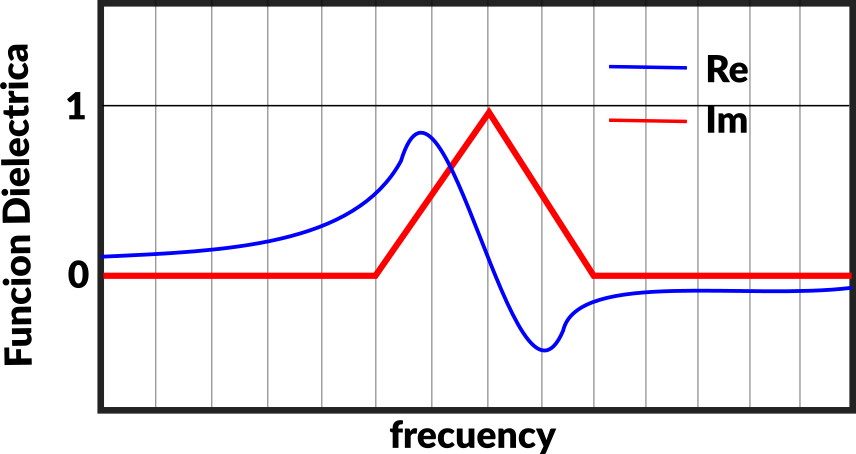
\includegraphics[width=250px, height=130px]{fd1.png}\\
\caption{Función dieléctrica triangular.} 
\label{FuncionTriangular}
\end{center}
\end{figure}




Ahora podemos construir la función variacional en nuestro caso la reflectancia como una superposición lineal de funciones triangulares por partes $R_{k}^{\bigtriangleup}$ localizadas a frecuencias fijas $w^{malla}_{k}$ (Figura \ref{FuncionVariacionalTriangular})\cite{constrained}.

\begin{equation}
\hat{R}^{\bigtriangleup var}(w^{malla})=\sum_{k=1}^{N-2}A_{k}\hat{R}_{k}^{\bigtriangleup}(w_{k}^{malla})
\end{equation}

Entonces $R(w_{k}^{malla})^{\bigtriangleup var}$ sera una curva a pedazos que pasa por los puntos $w_{k}^{malla},A_{k}$. Donde los parámetros $A_{k}$ dan forma a $R_{k}^{\bigtriangleup}(w_{k}^{malla})$ y de manera simultanea a $\phi_{k}^{\bigtriangleup}(w_{k}^{malla})$ ya que:

\begin{equation}
\hat{\phi}^{\bigtriangleup var}(w^{malla})=\sum_{k=1}^{N-2}A_{k}\hat{\phi}_{k}^{\bigtriangleup}(w_{k}^{malla})
\end{equation}  


\begin{figure}[H]
\begin{center}
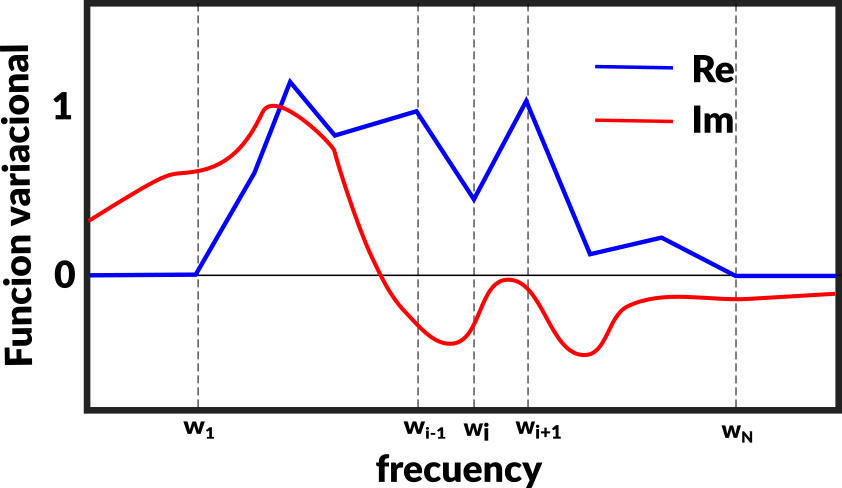
\includegraphics[width=300px, height=150px]{fd2.png}\\
\caption{ Función variacional}
\label{FuncionVariacionalTriangular}
\end{center}

\end{figure}

Por lo que cualquier forma experimental de $R_{i}(w_{i})$ puede ser representada  por un conjunto apropiado de parámetros $A_{k}$.
Para realizar el ajuste de parámetros y encontrar la mejor aproximación entre la función variacional y los datos ópticos experimentales debemos utilizar la técnica de mínimos cuadrados y construir el funcional $\chi^{2}$ \cite{guide}:\\

\begin{equation}
 \chi^{2}(\{R_{k}(w_{k})\})=\sum_{k=1}^{N-2}(\frac{R_{k}^{\bigtriangleup var}(w_{k}^{malla})-R_{k+1}(w)}{\delta R_{k+1}})^{2}
\end{equation}

El modelado sera esencialmente la minimización de $\chi^{2}$. Utilizaremos una minimización estándar no lineal, en particular el algoritmo ``Levenberg-Marquardt", el cual permite un balance auto ajustable entre dos técnicas de minimización ``El gradiente descendente", y el ``Inverso Hessiano" de manera que proveen de manera muy eficiente minimizar $\chi^{2}$ cuando el numero de parámetros es grande. Debemos tener en cuenta que la minimización de $\chi^{2}$ no debe causar un incremento fuera de cierto limite permitido, por lo que haremos uso de los llamados "limites de confianza". De esta manera obtendremos la mejor aproximación a la función dieléctrica. \cite{guide} 

Algo que debemos tener en cuenta es que la función de reflectancia modelo ignora complementa mente el espectro mas allá del rango de frecuencias experimentales limitado($w_{1} <w_{k}^{malla} <w_{N}$). Por lo que deberán tomar algunas consideraciones en el futuro, si se desea modelar el la función compleja mas allá del espectro medido. Entonces si el modelo de función de la reflectancia $R_{k}^{\bigtriangleup}(w_{k}^{malla})$ describe la mayor parte de las características del espectro entonces podemos asumir que la función da una correcta aproximación. En el caso en que debemos expandir el rango de frecuencia se debe agregar una función variacional adicional\cite{guide}:

\begin{equation}
R_{k}^{\bigtriangleup var}(w_{k}^{malla})=R_{k}^{\bigtriangleup var}(w_{k}^{malla})+R_{k}^{\bigtriangleup extra}(w_{k}^{malla})
\end{equation}

Por lo que se añade $R_{k}^{\bigtriangleup extra}(w)$ a $R_{k}^{\bigtriangleup var}(w)$, que es la contribución dominante a la reflectancia \cite{guide}.\\


\chapter{Desarrollo e implementacion}
En las secciones anteriores, se dieron los conceptos que envuelven la funcion dielectrica. Ahora es tiempo de continuar con el proyecto. Se construira una aplicacion web llamada Fafit que permitira lo siguiente:
\begin{itemize}
\item Desplegar una lista de las funciones dielectricas modeladas en la aplicacion y que son publicadas por usuarios a esta lista se llamara OpticStore.
\item Los usuarios pueden autenticarse
\item Los usuarios autenticados podran modelar la funcion dielectrica a partir de datos opticos medidos por la tecnica de reflectancia a incidencia normal de la superficie a una muestra de material.
\item Los usuarios autenticados pueden dar me gusta y comentar las funciones dielectricas publicadas en la opticStore.
\item Cambios en tiempo real cuando los otros usuarios dan me gusta o comentan, y tambien cuando se crean nuevos modelos de funcion dielectrica.
\end{itemize}

Para lograr esto se usaran las siguientes tecnologias para construir la app.

En el Frontend(En el lado del cliente):

\begin{itemize}

\item ReactJS: es una biblioteca JavaScript de codigo abierto para crear interfaces de usuario con el objetivo de desarrollar aplicaciones en una sola pagina. Es matenido por Facebook, Instagram y una comunidad de desarrolladores independientes y companias.
\item Relay: es el cliente GraphQl que utiliza Facebook y es  de codigo abierto desde 2015. Incorpora todos el aprendizaje que Facebook recolecto desde que empezaron a usar GraphQl en 2012. Relay es altamente optimizado para el desempeno y trata de reducer el trafico de red donde es posible. Los beneficios de relay vienen con un alto costo en la curva de apredizaje, relay es un framework complejo y entender todas sus partes requiere algun tiempo \cite{relay}.
\end{itemize}

En el Backend(lado del servidor):

\begin{itemize}
\item Graphcool: plataforma flexible que combina GraphLl+Sin servidor
\end{itemize}

\section{Casos de Uso}
Ahora se debe especificar la secuencias de acciones en el sistema que producen el modelado de la funcion dielectrica para ello presentamos el diagrama de casos de uso de la aplicacion:

\begin{center}
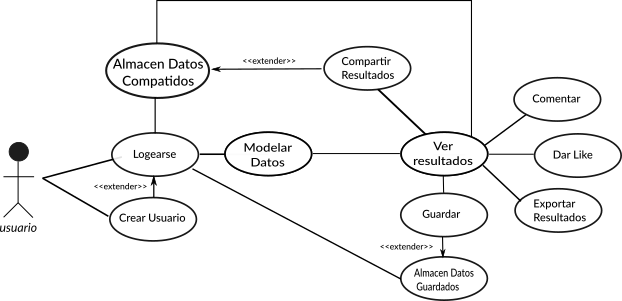
\includegraphics{diagramaCasoUso.png} \newline
Figura X. Diagrama caso uso Fafit.\\
\end{center}

Entonces pasemos a especificar cada caso de uso en mas detalle:\newline

\begin{table}[h]
\centering
\caption{Caso Uso Logear}
\label{my-label}
\begin{tabular}{|l|l|}
\hline
Nombre        & Logear Usuario                                                                                                                                                                                                                                                                                      \\ \hline
Descripcion   & \begin{tabular}[c]{@{}l@{}}El usuario provee su  correo y password para que sea autenticado por \\ el sistema\end{tabular}                                                                                                                                                                          \\ \hline
Actores       & Usuario                                                                                                                                                                                                                                                                                             \\ \hline
Pre-Condicion & ninguna                                                                                                                                                                                                                                                                                             \\ \hline
Flujo         & \begin{tabular}[c]{@{}l@{}}1) Ingresa a pagina de logeo.\\ 2) El usuario ingresa su correo y password \\ 3) Envia los datos\end{tabular}                                                                                                                                                            \\ \hline
Extension     & \begin{tabular}[c]{@{}l@{}}Si uno  de los campos esta vacio regresa a pagina de logeo mostrando \\ el error en el campo.\\ Si alguno de los datos no es correcto, regresa a la pagina de logeo y \\ despliega el mensaje de error informando que el correo o password\\ es incorrecto.\end{tabular} \\ \hline
\end{tabular}
\end{table}

\begin{table}[h]
\centering
\caption{Caso Uso Crear Cuenta}
\label{my-label}
\begin{tabular}{|l|l|}
\hline
Nombre        & Crear cuenta de Usuario                                                                                                                                                                                                                                                                                      \\ \hline
Descripcion   & \begin{tabular}[c]{@{}l@{}}El usuario provee su nombre, correo y password para que sea registrado\\ en el sistema\end{tabular}                                                                                                                                                                          \\ \hline
Actores       & Usuario                                                                                                                                                                                                                                                                                             \\ \hline
Pre-Condicion & ninguna                                                                                                                                                                                                                                                                                             \\ \hline
Flujo         & \begin{tabular}[c]{@{}l@{}}1) Ingresa a pagina de registro.\\ 2) El usuario ingresa su nombre de usuario, correo y password \\ 3) Envia los datos\end{tabular}                                                                                                                                                            \\ \hline
Extension     & \begin{tabular}[c]{@{}l@{}} Si el campo correo esta vacio regresa a pagina de registro mostrando \\ el error en el campo.\end{tabular} \\ \hline
\end{tabular}
\end{table}

\begin{table}[h]
\centering
\caption{Caso Uso Modelar la Funcion Dielectrica}
\label{my-label}
\begin{tabular}{|l|l|}
\hline
Nombre        & Modelar Funcion Dielectrica                                                                                                                                                                                                                                                                                      \\ \hline
Descripcion   & \begin{tabular}[c]{@{}l@{}}El usuario debe rellenar el formulario para crear un nuevo modelo\\ de funcion dielectrica, para ello debe indicar un nombre a los datos,\\ una descripcion y cargar un archivo con los datos opticos a modelar\\ \end{tabular}                                                                                                                                                                          \\ \hline
Actores       & Usuario                                                                                                                                                                                                                                                                                             \\ \hline
Pre-Condicion & Logearse al sistema                                                                                                                                                                                                                                                                                             \\ \hline
Flujo         & \begin{tabular}[c]{@{}l@{}}1) Indica el nombre de los datos, descripcion y el archivo de datos.\\ 2) Una vez cargado los datos pueden ser visualizados graficamente \\ 3)Luego se habilita el boton "Modelar" para asi analizar los datos y obtener la\\ funcion dielectrica asociada\end{tabular}                                                                                                                                                            \\ \hline
Extension     & \begin{tabular}[c]{@{}l@{}}ninguna\end{tabular} \\ \hline
\end{tabular}
\end{table}


\begin{table}[h!]
\centering
\caption{Caso Uso Analisis Kramers Kronig(KK)}
\label{my-label}
\begin{tabular}{|l|l|}
\hline
Nombre        & Analisis Kramers Kronig
\\ \hline
Descripcion   & \begin{tabular}[c]{@{}l@{}}El usuario luego de cargar el archivo de datos \\ la aplicacion podra analizar los datos cargados y modelar\\ la funcion dielectrica\\ \end{tabular}                                                                                                                                                                          \\ \hline
Actores       & Usuario                                                                                                                                                                                                                                                                                             \\ \hline
Pre-Condicion & Logearse al sistema                                                                                                                                                                                                                                                                                           ,Cargar archivo de datos \\ \hline
Flujo         & \begin{tabular}[c]{@{}l@{}}1) Luego que haya culminado el analisis mostrar en respectivas graficas\\ la funcion dielectrica generada(parte real y parte imaginaria)\\ 2) El usuario podra compartir los resultados en la opticStore, exportarlos\\ de manera local, o guardar en el almacen de resultados privados\\ de la aplicacion \\ \end{tabular}                                                                                                                                                            \\ \hline
Extension     & \begin{tabular}[c]{@{}l@{}}Si existe algun error en el proceso de analisis mostrar la advertencia con\\ el error que se produjo\\\end{tabular} \\ \hline
\end{tabular}
\end{table}


\begin{table}[h!]
\centering
\caption{Caso Uso Guardar}
\label{my-label}
\begin{tabular}{|l|l|}
\hline
Nombre        & Guardar Datos Opticos
\\ \hline
Descripcion   & \begin{tabular}[c]{@{}l@{}}Una vez modelada la funcion dielectrica \\ el usuario podra guardar la informacion obtenida dentro de la aplicacion web\\ \end{tabular}                                                                                                                                                                          \\ \hline
Actores       & Usuario                                                                                                                                                                                                                                                                                             \\ \hline
Pre-Condicion & Logearse al sistema                                                                                                                                                                                                                                                                                          ,Cargar archivo de datos, Modelar la funcion dielectrica \\ \hline
Flujo         & \begin{tabular}[c]{@{}l@{}}1)Guardar la funcion dielectrica generada\\ 2)El usuario podra observar las funciones dielectricas modeladas dentro \\de la aplicacion web en el almacen de resultados privado\\\end{tabular}                                                                                                                                                            \\ \hline
Extension     & \begin{tabular}[c]{@{}l@{}}\end{tabular} \\ \hline
\end{tabular}
\end{table}

\begin{table}[h!]
\centering
\caption{Caso Uso Exportar Resultados}
\label{my-label}
\begin{tabular}{|l|l|}
\hline
Nombre        & Exportar resultados del Analisis KK
\\ \hline
Descripcion   & \begin{tabular}[c]{@{}l@{}}Una vez modelada la funcion dielectrica \\ el usuario podra exportar localmente la funcion dielectrica modelada\\ \end{tabular}                                                                                                                                                                          \\ \hline
Actores       & Usuario                                                                                                                                                                                                                                                                                             \\ \hline
Pre-Condicion & Logearse al sistema                                                                                                                                                                                                                                                                                          ,Cargar archivo de datos, Modelar funcion dielectrica \\ \hline
Flujo         & \begin{tabular}[c]{@{}l@{}}1)Exportar localmente la funcion dielectrica modelada en dos archivos\\ uno para la parte real y otro para la parte imaginaria\\ \end{tabular}                                                                                                                                                            \\ \hline
Extension     & \begin{tabular}[c]{@{}l@{}}\end{tabular} \\ \hline
\end{tabular}
\end{table}

\begin{table}[h!]
\centering
\caption{Caso Uso Compartir en la opticStore}
\label{my-label}
\begin{tabular}{|l|l|}
\hline
Nombre        & Compartir resultados en la opticStore
\\ \hline
Descripcion   & \begin{tabular}[c]{@{}l@{}}Una vez modelada la funcion dielectrica \\ el usuario podra compartir los resultados publicamente en la opticStore\\ \end{tabular}                                                                                                                                                                          \\ \hline
Actores       & Usuario                                                                                                                                                                                                                                                                                             \\ \hline
Pre-Condicion & Logearse al sistema                                                                                                                                                                                                                                                                                          ,Cargar archivo de datos, Generar funcion dielectrica \\ \hline
Flujo         & \begin{tabular}[c]{@{}l@{}}1)Compartir la funcion dielectrica generada\\ 2)Los demas usuarios podran ver la funcion dielectrica publicada \\\end{tabular}                                                                                                                                                            \\ \hline
Extension     & \begin{tabular}[c]{@{}l@{}}\end{tabular} \\ \hline
\end{tabular}
\end{table}
\clearpage

\section{Diagrama de actividades}
En Lenguaje Unificado de Modelado (UML), un diagrama de actividades representa los flujos de trabajo paso a paso de negocio y operacionales de los componentes en un sistema. Un diagrama de actividades muestra el flujo de control general. Se generá un diagrama de actividades por cada caso de uso.

Para un usuario que se registra en el sistema
\section{Diagrama de secuencia}
\section{Arquitectura}
\section{Modelo de datos}
El modelo de datos se escribira en el lenguaje de definicion de esquemas de GraphQL(Schema Definition Language) ya que es la manera mas concisa de especificar un esquema GraphQL:

\begin{center}
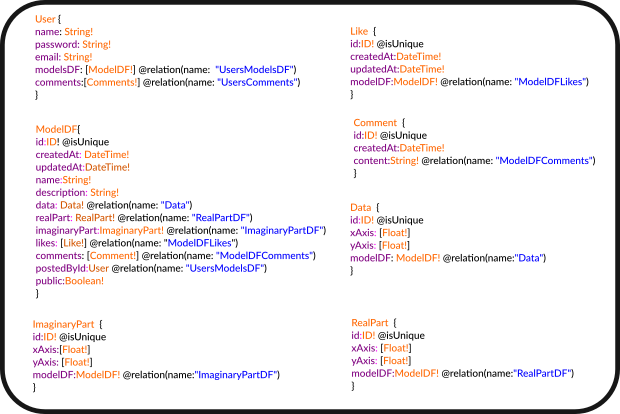
\includegraphics{modeloDatos.png} \newline
Figura X. Esquema de datos Fafit.\\
\end{center}
En forma de diagrama que represente las relaciones uno a uno y uno a muchos tenemos que para fafit es:
\begin{center}
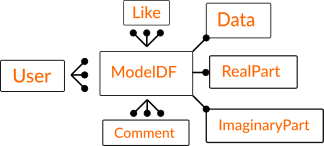
\includegraphics{diagramaDatos.png} \newline
Figura X. Diagrama de datos Fafit.\\
\end{center}

\bibliographystyle{ieeetr}

\bibliography{bibliografia}



\end{document}




